\documentclass[]{report}
\usepackage[utf8x]{inputenc}
\usepackage{hyperref}
\usepackage{changepage}
\usepackage{graphicx,subfigure}

% Title Page
\title{Lessons learned at LLNL}
\author{Zachary Matheson}


\begin{document}
\maketitle

\section*{Nucleon localization function}
\subsection*{\date{1 March 2017}}
Most recently I tried using Erik's modified version of HFBTHO to run for several constraints along $Q_{30}$ (or anywhere, really). What I'd like to do is use HFBTHO to generate densities quickly for $^{176}$Pt between $Q_{20}=241$ and $Q_{20}\approx 300$, and at $Q_{30}=4, 18$ (something I decided semi-arbitrarily once upon a time). I'm putting that on hold for a bit while I work on this inertia thing. Erik sent me some notes for perhaps getting the code to do what I want it to do, which are in my email. The files are currently in /p/lscratchh/matheson/locali-176Pt/hfbtho (/erik for testing his version of the code). Another thought I had was to try constraining $Q_{40}$ to something reasonable, and then releasing that constraint to find the actual density (hopefully) nearby.

\subsection*{17 May 2017}

Okay, I finally have some localizations worth talking about. I ended up settling on $^{176}$Pt, going along the axes $Q_{30}=6$ and $18$. Then once I got close to scission (and things started having trouble converging), I turned off the constraint on $Q_{30}$ thinking that would perhaps help with convergence and also round to fragments with the nearest whole number of particles. And it seems to have somewhat worked.

The more mass-asymmetric case ended up shifting from $Q_{30}=18$ to a little over 20, which is fine, though it should be noted that those calculations failed to converge and I'm not totally sure why. But taking them as fully-converged, correct solutions (in any case, I expect the densities to be pretty close to reality), we produce the fragments $^{93}$Nb, with an elongation $Q_{20}\approx3-5 b$, and $^{83}$Rb, with an elongation $Q_{20}\approx10-15 b$ (both fragments also show a small mass asymmetry of less than $1 b^\frac{3}{2}$, no doubt due to the heavy interactions between the two non-yet-fully-independent fragments). The weirdness of those two fragments leads me to wonder if perhaps I released the $Q_{30}$ constraint too late in the development of fragments, such that those fragments were determined (according to Nicolas's fission fragment toolkit in HFODD), \textit{at least} by $Q_{20}=285 b$, and probably well-before that.

In the more mass-symmetric case (but still with $Q_{30}\neq0$), it actually appears that the system chose to produce two equal-mass fragments ($^{88}$Y), and then to just deform one of them more than the other. So even though their mass and charge distribution is symmetric, the kinetic energy distribution is not.

Now, what I'm wondering is what is the benefit to all of this? I think the goal was that it would be nice to be able to identify fission fragments well before scission. Well, let's look at the output files I actually saved (why did I not think to save them all?! $\frown$). In the symmetric case, at $Q_{20}=285b$, the calculation actually failed to converge because the number of iterations was reached. But we did get an output, and according to that output the ``prefragments'' at that stage were $^{96}$Tc and $^{80}$Br. $Q_{20}=300b$ also failed to converge, and also gives two asymmetric fragments ($^{91}$Nb and $^{85}$Rb, but the localization plots \textit{look} symmetric, in case that means anything). When I got around to doing $Q_{20}=315b$, the fragments are actually \textit{still} not symmetric (according to the fragment toolbox) (I'll just print the output here):
\begin{verbatim}
*   -----------------------------------------------------------------------   *
*             |   LEFT  FRAGMENT (z < zN)   |   RIGHT FRAGMENT (z > zN)       *
*   -----------------------------------------------------------------------   *
*       <A>   |          88.9232            |          87.0768                *
*       <Z>   |          39.4393            |          38.5607                *
*       Etot  |         -33.0708            |         -46.1156                *
\end{verbatim}

\noindent And looking at the localization, you get the sense that it's going to be a \textit{fairly} even split, but you can't be totally sure because there are still some subtle differences between the two halves.

Okay, well, let's hold on here. Say we take these, and we have some sense of what the fragments are likely to be so we plot those as well. And then we sort of ``overlap'' the fragments and see if it matches up with the parent. So the way you could do this is to run calculations for several fragments in the region near where you expect fragments to appear, and give them the deformations you expect them to have at scission, and see if you can distinguish between the various fragments: do they have distinct clustering structure? Or perhaps some kind of unique shell-looking behavior?

\subsection*{18 May 2017}

Just by way of update on the mass-symmetric(-ish) case: I brought the quadrupole deformation out to 400 and still no signs of splitting. The properties of the fragments are equilibrating so perhaps it won't scission until it is able to conserve energy by doing so? Which would probably mean redistributing energy amongst the particles for a bit longer and then it'll be ready to break apart.

\subsection*{28 September 2017}

Apparently I never wrote about this before, but I wanted to test just \textit{how} distinct fragment shell structures were, and whether you'd be able to identify the fragments based on the localization. So I looked at a few possible fragmentations of $^{176}$Pt, just to see what we could learn. Here I'll show the proton localization plots for the lighter fragment as an example (the rest are stored on my computer somewhere). The fragments I chose to show (based on some semi-arbitrary fragment trajectory in the PES) were $^{82}$Se, $^{84}$Se, and $^{86}$Zr. $^{84}$Se has a magic number of neutrons (N=50); $^{82}$Se is two neutrons shy of a full shell; and $^{86}$Zr, with Z=40 and N=46, is not particularly close to a full shell in either nucleon.

\begin{figure}
  \begin{center}
    \subfigure[$^{86}$Zr]{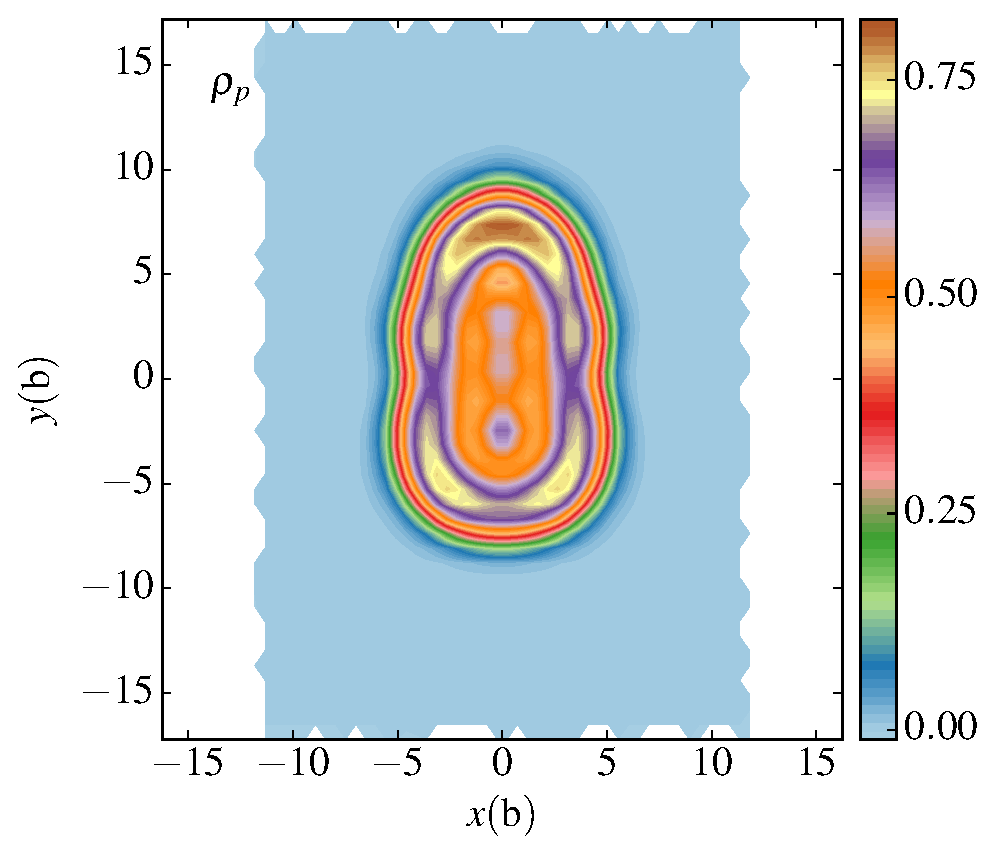
\includegraphics[width=0.3\linewidth]{86Zr-p-locali.eps}}\label{fig:86Zr-p-locali}
    \subfigure[$^{84}$Se]{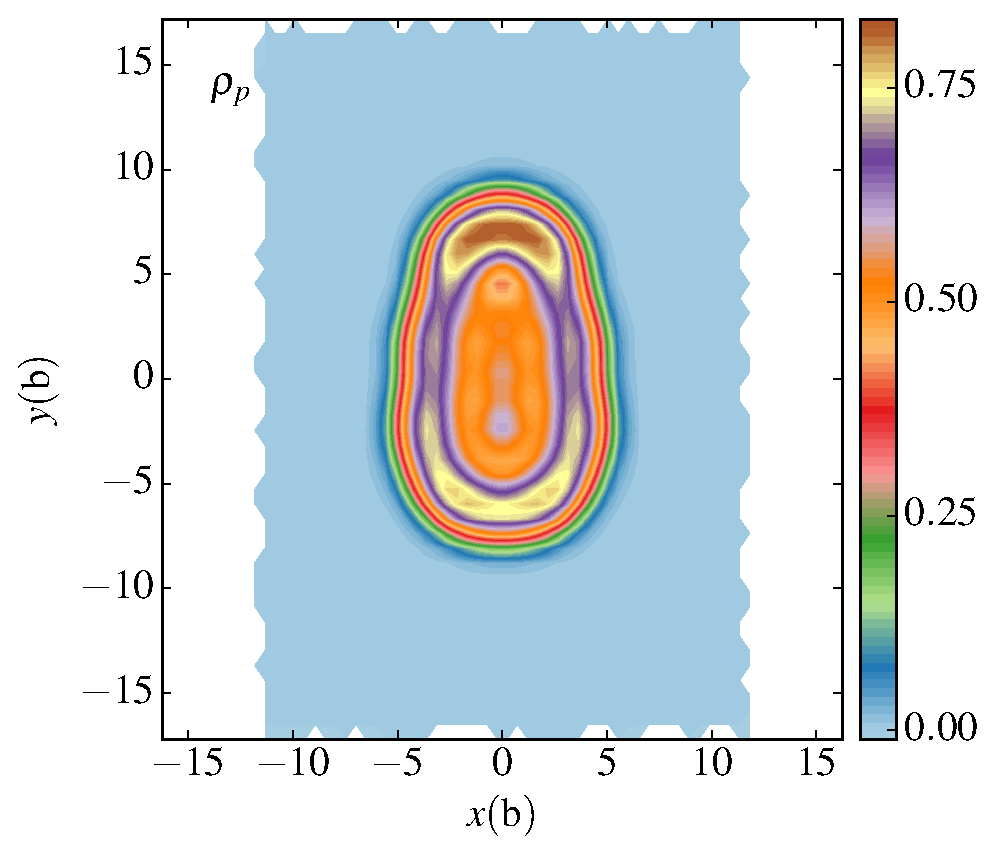
\includegraphics[width=0.3\linewidth]{84Se-p-locali.eps}}\label{fig:84Se-p-locali}
    \subfigure[$^{82}$Se]{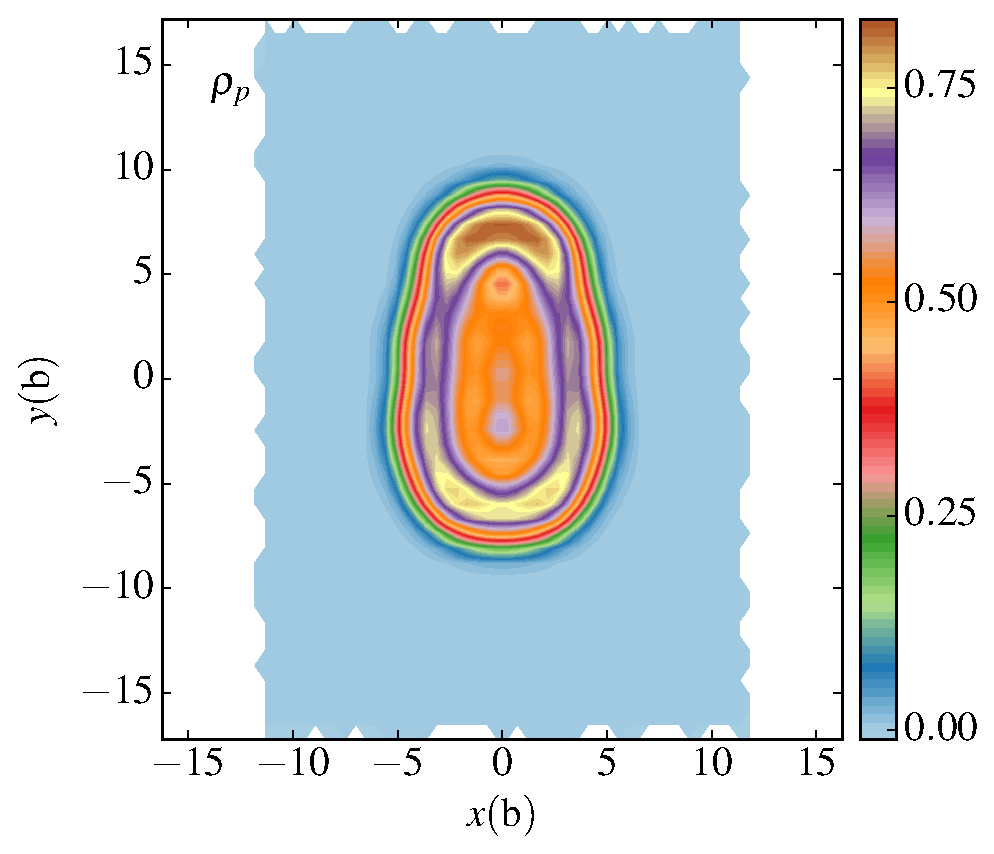
\includegraphics[width=0.3\linewidth]{82Se-p-locali.eps}}\label{fig:82Se-p-locali}
  \end{center}
  \caption{Proton spatial localization}
\end{figure}


As you can see, at this level, the selenium isotopes are virtually indistinguishable. Of course, that should not be surprising, as the number of protons stays the same. However, even looking at the neutron spatial localizations doesn't change the conclusion too much. The signatures are different but I don't know if they're so distinct that I'd be able to distinguish between them in a pre-scission developing fragment.

$^{86}Zr$ is distinct from the seleniums (as it should be, given that it differs by 6 protons). That said, I again don't know that I'd be able to pick them apart in a prefragment. Maybe.

\section*{Impact of basis deformation on $E_{HFB}$}
\subsection*{\date{1 March 2017}}
We wanted to see how much the observables of the system would change if we used a single HO basis across an entire PES. This is based on a misunderstanding I had of something Jhilam said, where in order to use his inertia code, you need adjacent points to have the same basis deformation and other basis properties (so that you can numerically take derivatives of the densities at those points). It turns out he gets around this problem by changing the basis every 30b along Q20, but all the same we thought it would be good to check the dependence of system observables on the basis, especially since the half-life is so dependent on small deviations in the potential energy (a change of 1 MeV can affect the half-life by orders of magnitude).

To test, I took three points on the PES I had generated for $^{294}$Og: (-14, 0), (72, 0), and (148, 28). According to the output file, the basis deformation chosen for each of these (by the automatic basis setting routine in HFODD) was, respectively, AL20 = 0.187, 0.424, and 0.608. I took those record files and used them to restart a new calculation, this time with the basis deformation set uniformly to AL20 = 0.61 (and AL40 = 0.10). The superdeformed asymmetric shape was, understandably, least affected by the change, with the kinetic energy varying by about 3 MeV but the total energy varying by only about 0.14 MeV (-2085.878548 vs -2086.012955). Quasiparticle and canonical single-particle states were nearly identical, and fragment properties were almost the same (except for the interaction energies, which were quite different). The elongated symmetric shape differed by about 0.6 Mev (-2080.815396 vs -2080.202346). The oblate ground state didn't converge in the allotted time, but based on its last iteration it was probably going to finish with an HFB energy around -2078.649984 (compared to -2080.263986 from before), a difference of about 1.6 MeV.

\subsection*{3 March 2017}
I've written a Python script which extracts the basis parameters from a previous run of HFODD, and uses it to initialize a new run for several neighboring points in order to facilitate an inertia calculation down the line. A problem we noticed, though, was that, while setting the $\alpha_2$ deformation parameter worked fine, the basis was totally different because there was an additional constraint on $\alpha_4$. It turns out that what had happened is that the code automatically sets default values of $\alpha_2$ and $alpha_4$, UNLESS you set the code to choose the basis automatically, in which case it only sets a value for $\alpha_2$. You can get around that by deleting the preset line in HFODD and recompiling, but I'd like for there to be an easier way. Perhaps the basis matrix is initialized to zero? So we could get around it by just setting $\alpha_4=0$ in the input file? $\Rightarrow$ Aha, yes. That'll work. So we're benchmarking the time on that now.

Another thing we're testing is comparing versions of the inertia code. Jhilam sent Nicolas an input and an output for $^{240}$Pu. I'm running a single point now. Later, I'll run the surrounding points using both my convention and Jhilam's for how widely-spaced the points should be. I'll also compare the inertia computer with the code Jhilam sent me versus the one in Nicolas' repository.

Unfortunately, this run uses Lipkin-Nogami, and for some reason the parser doesn't write the data to the XML file, which ultimately means I'm going to have to set up the subsequent runs by hand. The question is whether to do so using Jhilam's convention (for benchmarking purposes) or the one Nicolas and I talked about (where the points are much closer and you might get a better value for the inertia). Computing the neighboring runs will probably still take a similar amount of time (it took roughly 50-60 iterations for a deviation of about 0.001 units in each direction. It'll probably be more for something farther away but if you already have those computed anyway it might not be such a big deal).

So I went ahead and did that. Once those jobs complete, we can try to analyze the inertia using each of the inertia codes, just to make sure they both give the same results. I used Jhilam's grid spacing, but we can try it again later with the narrower grid spacing once we see how long it takes for these points (which have a grid spacing of 1 in the multipole constraints, and 0.1 in the pairing constraints) to converge and then decide if using the narrower grid is economical and useful. Actually, this would be a good test case for that; if we see a noticeable improvement in accuracy, then the extra time-to-solution for the narrower grid might be worthwhile.

Of course, to do that we'll need working inertia codes. Right now, I don't undertand why, but for some reason we're getting some kind of runtime error in LAPACK:

$\mathtt{Intel MKL ERROR: Parameter 8 was incorrect on entry to ZGEMM}$

\subsection*{6 March 2017}
Today I worked on two computational problems: the large number of iterations, even for a small perturbation from the record file's original point; and benchmarking a working inertia calculation against Jhilam's results.

For problem \#1, I noticed that even after setting the basis parameters manually in the input file, I was still seeing that a different basis was used during the run and [consequently?] these were still taking ~70-80 iterations to converge. I showed Nicolas and he had me flip a Lagrange multiplier continuation switch in the input file, but I've re-run the code since then and the problem still exists, that the new run uses a slightly different basis than the original. and it still takes ~70-80 iterations to converge.

For problem \#2, I compiled the code for a 3D benchmarking run to compare with Jhilam's results. The code runs without that weird MKL error I was getting, but the results are incorrect.

I'm getting:
\begin{equation}
   77.00\    1.00\    2.00\   -1801.146627 \\
       0.000000\    0.598205\    0.598233\    0.000000\    0.000000\    0.598219
\end{equation}
whereas Jhilam is getting:
\begin{equation}
   77.00\    1.00\    2.00\   -1801.183 \\
   0.010463\    0.033608\    0.000842\   -0.001305\   -0.000412\    0.000152
\end{equation}

\subsection*{7 March 2017}
Today, after modifying the input file and doing some debugging, I'm getting:
\begin{equation}
    0.011378\    0.034354\    0.000000\   -0.001988\    0.000000\    0.000000
\end{equation}
\noindent which is within 0.001 across the board. So not bad, but not exact, either. My question now then is if this is something that should be exactly deterministic. I'd think that it should be, yes. The max basis size has changed at compile time but I don't think that affects the final results. $\Rightarrow$ Ah. I think the problem is that I changed the basis characteristics in the input file to HFODD. I calculated the surrounding points using the basis from the centerpoint. Which, I suppose is useful to know... In fact, yes, I did that because we need the basis to be the same, no? So in order to reproduce Jhilam's exact results, we'd need to know his exact basis.

Pending that, I think I officially have a working inertia code. There are some nice things I can do to streamline inertia calculations, probably within Python as opposed to Fortran, but for now it's something to start with.

I'm still not sure what's going on with the other thing, with the basis getting changed even after setting it manually. I even tried another run setting INPOME=0, just to see what would happen (even though I expected that to make it worse), and frankly I didn't see a difference (the output files reported the same wrong basis).

When you come in tomorrow, the things to work on should be: 1) spend the morning working on deriving the ATDHFB inertia, then 2) in the afternoon, talk to Nicolas about the inertia code you got working (maybe Jhilam will have sent you a basis to use), and perhaps see if Nicolas has any additional insight on the basis problem you're seeing here.

\subsection*{8 March 2017}
Good news: Nicolas figured out what was happening with the basis. Apparently there were rounding truncation errors that popped up when the parameters FCHOM0 and AL20 were written to file, and the line FREQBASIS isn't even read at all. Going back into the source and figuring out how FCHOM0 and AL20 were computed for the centerpoint, and plugging these values into the input file with lots of decimal points seems to have solved the problem. It still takes several iterations to converge, but it will hopefully be faster than before (it's still running so we'll see).

The formulae you'll ultimately need to implement in your Python script for preserving the basis are the following:

\begin{eqnarray}
\omega_0        =& 0.1q_{20}e^{-0.02q_{20}}+6.5 \\
\mathtt{FCHOM0} =& \frac{\omega_0}{\left(\frac{41}{A^\frac{1}{3}}\right)} \\
\alpha          =& 0.05\sqrt{q_{20}}
\end{eqnarray}
\noindent where $q_{20}$ refers to the quadrupole deformation of the centerpoint.

\subsection*{9 March 2017}
Aha! Figured out what was causing the ZGEMM error in the inertia file. I was using a max basis size of 1200 when I compiled the inertia code (as defined in hfodd\_sizes\_....f90), but the particular matrices I was trying to multiply were created using a basis size of like 1600. So that's resolved. One thing, though, is that, while it gives the same results as the 3D case, they are in a different order. So that's something you should clean up in the code. 

Additionally, I've redone the calculations for the inertia benchmark, this time using the correct basis for the points surrounding the center point, and fixing whatever Lipkin-Nogami problem I was having, and this is what I get:
\begin{equation}
    0.011719\    0.034843\    8.287077\   -0.002180\   -0.054160\    0.020690
\end{equation}
\noindent with $E_{HFB}=-1801.146627$ Again, for reference, here are Jhilam's results:
\begin{equation}
   0.010463\    0.033608\    0.000842\   -0.001305\   -0.000412\    0.000152
\end{equation}
Without Jhilam's basis, we still don't have his result (in fact, it's even further than it was before). But the biggest problem is in that $\lambda$ variation somehow. Still not sure what's going on with that.

Just judging from the outputs, it looks like everything converged properly and the results make sense (energies were approximately the same, particularly for those which did not explicitly involve pairing; unconstrained multipole moments are approximately the same as far as I can see). Could it be that I put the qp files out of order? I have the magnitudes right for sure (lambda changes by 0.01; the Lagrange coefficient magnitudes for equally-spaced grid points go as $\pm\frac{1}{2\delta q} = \frac{1}{0.02}=50$). I'm running it now with the signs switched, just in case I had them backwards somehow. 

\begin{equation}
    0.011719\    0.034843\    8.287077\   -0.002180\    0.054160\   -0.020690
\end{equation}

\noindent But if that doesn't work (which it didn't), then perhaps it's a problem related to the parameter I switched? Is there a modification to the formula when you change $\lambda$ instead of a multipole moment? Did I change the wrong $\lambda$? Was I only supposed to change $\lambda$ for protons $\mathit{or}$ neutrons but not both?

\subsection*{10 March 2017}
Okay, I have information about the basis Jhilam apparently used: for $Q_{20}=77$, he would have used the basis corresponding to $Q_{20}=60$ (as far as FCHOM0 and $\alpha_{20}$ are defined). In general, his method is to round down to the nearest multiple of 30. With this I get:

\begin{equation}
    0.011663\    0.034763\    8.610518\   -0.002182\   -0.054110\    0.020785
\end{equation}

\noindent with $E_{HFB}=-1801.173695 MeV$

\subsection*{13 March 2017}
It seems there's no problem with the $\lambda$ terms in the inertia output (at least, not one unique to just the pairing terms).  The issue there is that Jhilam normalized his coordinates in the end, such that $\delta x=1$ for every collective coordinate instead of the $d\lambda=0.01$ I'm using. Since this only affects the denominator in my derivatives $\frac{\delta \rho}{\delta q}$, this means shifting the decimal point over by 2 slots (or 4 in the $\lambda-\lambda$ case) for the pairing terms.

So it $\mathit{looks}$ like the inertia code is working. Everything is correct to within ~20\% compared to Jhilam's result. But it would be good to make absolutely sure, which means examining Jhilam's output files, if possible. 

\section*{Inertia Wrapper}
\subsection*{17 March 2017}
The past couple days you've been working on parallelizing the inertia routine, and figuring out how to quickly setup runs for the "satellite" points on your PES. You've got some scripts that will help, although between writing them a couple days ago and using them now, it seems you've already sort of forgotten what they need to work - or rather, you see that they aren't quite as universal as you were hoping. You need an XML file, which needs output files. If you have a big XML file and need to split it up, you did that by hand today but I'm guessing there's an easier way. But it looks like you WILL need to do some splitting up. Not the way you had originally anticipated, where you submitted a job for every single point on the PES to have its satellites computed. But since the speedup for using nearby points only seems to occur when you use the same basis as the centerpoint, this means that you have to group centerpoints by $Q_{20}$. That'll reduce the number of jobs on Quartz by ~15, but it's still a nuisance.

Anyway, you've done that for values of $Q_{20}$ between 0 and 8, and you're waiting for those to complete (hopefully they'll take less than 3hrs!). Once they do, you can test out your post-run\_whatever.py Python script to see if it really \textit{does} group things nicely. You should have it generate the inertia input file, with multipole moments, Lagrange coefficients, and file names correctly and automatically (it's mostly there already; I think you just need to add the multipole constraints). And then you can test out your MPI version of the inertia code. You've tested it and it works when compiled and run serially (at least, it gives the same results as before, which you'll assume are correct until you hear back from Jhilam).

\subsection*{21 March 2017}
When you get around to setting up your inertia wrapper, I think the nicest and most user-friendly thing you could do would be to activate the Python setup script.

\begin{enumerate}
\item It should take as inputs the XML file and the directories containing record, qp, and maybe output files (and Lipkin files if you're into that kind of thing).
\item[Note] Whatever naming scheme you use, it should be independent of the indexing scheme used originally.
\item It'll create and populate directories for each $Q_{20}$ value, create path and path\_new files for each directory that HFODD can use to calculate the neighbors.
\item Then it'll create the SLURM batch script (with multiple SRUN commands) that HFODD will use to compute the neighboring points.
\item Once HFODD is done, those same MPI ranks will collect the outputs into their proper folders with their proper names. Python will create input files for the inertia code in each subdirectory. Then it will run the inertia code on a subdirectory level.
\item After the inertia code completes on a subdirectory level, the results (and perhaps the output files if you're into that kind of thing) will be collected and compiled into the parent folder, and a master output file will be created.
\end{enumerate}  

\subsection*{28 March 2017}
I haven't really explained what I've been up to for the past several days (or at least, I haven't committed my thoughts from my notebook to my computer). After discovering that much of the inertia wrapper I was trying to develop had already been done more cleanly by Nicolas, this week I've started developing a new Python class called Point, which corresponds to a single point in the PES. I'm going to give it some neat methods that will sort of streamline the creation of neighboring jobs and such. Right now, I've successfully been able to initialize an instance of Point from an instance of DataFile (just by picking one of them out randomly). The script which was able to do that is the following:

\begin{verbatim}
from pes import * 
from collections import defaultdict,Counter
oldpoint = Point('294Og_PES.xml', 176, 118, var=('q20','q30'))
tree = oldpoint.ReadFile()
glob_dico = oldpoint.GetGlobal(tree)
dico = {}
dummy = oldpoint.GetVariable(tree, val='id')
dico['id'] = dummy['id']
for constraint in oldpoint.var:
	dummy = oldpoint.GetVariable(tree, val=constraint)
	dico[constraint] = dummy[constraint]
	
dico_arr = {}
for observable in ['EHFB', 'Z1', 'A1', 'zN', 'qN', 'D']:
	dummy = oldpoint.GetVariable(tree, val=observable)
	dico_arr[observable] = dummy[observable]
	
newpoint = oldpoint.CreateNewPoint(glob_dico, 0, oldpoint.var, dico, dico_arr, 0)
\end{verbatim}

One complication that arises, however, is that in order for this to work as currently written, the old point must be initialized from the entire XML file, and that XML file must currently be an element in the Point class (which technically is possible but it sort of violates the goal of the project). It would be nice to have a method which truly takes an actual DataFile and spits out a Point. What you might consider doing is generating a DataFile from a DataFile, and then taking the output DataFile and using it to initialize a Point afterwards. Anyway, something to think about.

\subsection*{29 March 2017}

Welp, it turns out I've been working on an outdated branch of the PES module. I got access to the latest one today and spent the afternoon familiarizing myself with what's new. It seems really nice and sleek, so I think it should be pretty easy to work with and adapt what I've been doing. Now I just need to spend some time figuring out what changes.

And I had \textit{just} gotten my instance of \texttt{Point} to initialize from a \texttt{DataFile}...

\subsection*{31 March 2017}

So the good news is I've created a successful Point class in the new \texttt{pes\_tools} module, and you can specify a set of constraints with their values and it'll spit out an XML tree for that particular point. You can also find neighbors surrounding that point as XML trees, the idea being that you can feed them into input files for use in an inertia calculation.

The thing is it all feels so stupid. It's been done already! Why does it need to be done again? Indeed, this will look a little bit cleaner, hopefully. Then your actual inertia\_setup script can probably be actually pretty short. You'll still have to deal with file movement, but a lot of things will be moved behind the scenes into the various pes module methods.

The toughest spot will be the part you've been avoiding the most: figuring out how to divide up a whole large reservation of processors to cover the entire PES efficiently and without overlap. You can fit 3 neighborhoods per node (assuming 4 neighbors per neighborhood and 3 OpenMP ranks per task = 12 tasks per neighborhood, with 36 possible tasks per node). Just FWIW, assuming something like 830 neighborhoods (which is roughly what you've got right now for $^{294}Og$), that's going to require $830/3 \approx 277$ nodes. Estimating walltime, I'd give yourself something like an hour and a half to two hours to do the HFODD run for the neighborhood, and another half hour to do the inertia calculation. Three hours \textit{should} be more than enough time to do it all. I say "should" because these SLURM emails sitting in my inbox report inertia calculation times closer to an hour and a half, for the HFODD portion, but they never actually completed the inertia calculation (I was trying to do them all at once, but it's probably best to just do it by neighborhood, rather than for a whole slice of neighborhoods).

Whatever script you end up creating, you should make it modular and flexible enough that you can pin a path calculation onto the end of it without too much trouble. And it should work in any number of dimensions (which thankfully, so far it does. Your other script would have taken some real tweaking for that to happen, though). The one place where this might struggle is when probing along the pairing parameter. I imagine you could tweak that, too, without it being a huge problem, but that's going to take some thought. Most likely everywhere you have a loop over \texttt{collective\_variables}, you'll need to stick an \texttt{if q == lambda\_n or q == lambda\_p} statement in there.

\subsection*{7 April 2017}
Holy crap, it's been another week! Welp, in any case, I think I'm going to give up trying to get MPI Spawn from within a Python script to launch HFODD runs. I've had some level of success. To pull this off, you needed to be able to launch several concurrent MPI tasks simultaneously, each with several OpenMP threads:

\begin{verbatim*}
Task 1 BB/__/__/__/__/__/__/__/__/__/__/__/__/__/__
Task 2 __/__/__/__/__/BB/__/__/__/__/__/__/__/__/__
Task 3 __/__/__/__/__/__/__/__/__/__/BB/__/__/__/__
\end{verbatim*}

That's all okay. We got that. Then you needed to spawn onto these processors. You were able to achieve something like that by using the option \texttt{--oversubscribe} (although it's not clear that the specially-designated processors were used properly). But the real issue is launching HFODD after that. To do it, you'd need to somehow launch another \texttt{srun} with a different number of \texttt{OMP\_NUM\_THREADS}. But to use MPI Spawn properly, you need the spawned process to establish, and later, disconnect from an MPI Communicator (otherwise the process will lag indefinitely). You could get around this by combining the two and spawning a process which calls a Python script (with the proper MPI communicators enabled and whatever) that launches an HFODD subprocess via \texttt{srun} (be sure to change the number of threads!). And you know, this might work... but at this point it's just seeming less and less reasonable. And I'm not sure you'd be spawning onto the correct, pre-reserved processors \textit{still}. I think you're better off in the long run just reserving a bunch of resources, and then launching a bunch of simultaneous \texttt{srun}s and letting the scheduler divide up the jobs itself. I feel like that's a lot simpler to implement, and probably a lot more portable in the end. To do \textit{this}, you'll need to write a Python script to handle the file management, and then refer to it in the batch script (you can do it in parallel still, I'm sure), followed by HFODD \texttt{srun}s, followed by either shell or Python file movement, followed by inertia \texttt{srun}s, followed by more file movement. So you might have 3 or 4 Python scripts: pre-HFODD, post-HFODD/pre-inertia, post-inertia, and a wrapper to write the batch script. That just feels so messy but it feels like the simplest way if you don't have the MPI Spawn (which was supposed to be the "One script to rule them all!"). I mean, I guess maybe the wrapper could write the other ones on the fly?

Just to reiterate and make it clear, though: \textbf{Spawning a multithreaded executable}... actually might work, IF you had a specially-made executable just for that purpose. The question is whether it's worth modifying HFODD. So my question is, for a spawned process, do calls to \texttt{MPI\_COMM\_WORLD} refer to the communicator created by the spawn (i.e. \texttt{MPI\_GET\_PARENT}) or everything from before? I'm inclined to believe that it should just be the stuff you care about. So you could probably get it to work by just adding a few lines \texttt{MPI\_Comm\_get\_parent( parentcomm )} right after MPI\_INIT and \texttt{MPI\_Comm\_free( parentcomm )} right before MPI\_finalize (tucked inside some preprocessor option, of course). That might work... Okay, that's my goal for the end of the day. Compile a version of HFODD that is meant to be a worker in an MPI\_spawn, and see if you can get it to run.

\noindent\textbf{UPDATE}

...Okay, I am officially declaring \textbf{MPI Spawn NOT the solution} that I'm looking for. When I set up a test run, there was some error. I didn't have time to diagnose it yet when I talked to Kyle and he pointed out that mixing MPI implementations will lead to all kinds of crashes. That means that since my Fortran executable was built using the default system MVAPICH while my Python launch script was running from a side installation of mpi4py built over OpenMPI, they were going to have issues talking to each other (which is probably what I saw). So no, that's not gonna happen.

\subsection*{10 April 2017}
I decided I'm going to try doing things the easy way: just making one large resource allocation request, and in the script submitting several srun commands in the background and letting the scheduler figure out how to spread them out. I think that'll be the easiest and most portable in the long run. Right now the issue I'm having is that I'd like to define and launch those srun commands within a Python script; however, the resource allocation closes when the tasks in the script complete, and any jobs launched in the background by Python are disconnected from the batch script which launched Python, with the result that the scheduler \textit{thinks} that the job has finished even though there are tasks running in the background. I could get around that by having one thread just sleep for a really long time, but that would waste a thread and also it'd waste a lot of walltime if there really was a problem in the executable somewhere that caused it to close early.

I ended up getting by it for the time being by just probing \texttt{ps} every 60 seconds, and if there is still an srun process running, the process sleeps for 60 seconds and tries again. I guess this isn't much better than having the one thread sleep for a long time since it still ties up a thread somewhere (which may or may not lead to a performance hit somewhere else? It's not resource intensive so it shouldn't be a big deal to multithread this on a processor with some other task...), but it does get you to within a minute of the actual execution time, so worst case scenario you waste about 59 seconds of walltime.

And with that, I have a launch mechanism! Thank heavens I can move on now! Now to build the rest of that Python launch script (not to mention finishing up those point-based utilities)...

And the nice thing is that this is fairly portable. For a system that uses mpirun/mpiexec instead of srun, you can chain jobs together like this:

\begin{verbatim}
shell$ mpirun -np 2 a.out : -np 2 b.out
\end{verbatim}

And in fact, you might even be able to do something fancier with srun by creating a MPMD config file:

\noindent\verb|https://computing.llnl.gov/tutorials/linux_clusters/multi-prog.html|

\subsection*{15 May 2017}

This isn't part of the wrapper, per se, but it is relevant to the development of the ATDHFB inertia code, and specifically the temperature-dependent implementation of it. The $T>0$ version of the code ends up getting \textit{HUGE} values for the inertia, even for small temperatures like $T=0.05$ which should be almost unchanged from the $T=0$ case. It's not a matter of accidentally dividing by zero when $f_a=f_b$ because the code explicitly filters those out. It's about the relative sizes of $\dot{\mathcal{R}}$ and $f_a$, or actually $\frac{\partial \mathcal{R}}{\partial q}$ and $f_a$. The code calculates both of these based on the HFB matrices and the quasiparticle energies stored in the .QP files. For the test case I looked at (which was a sample case of $^{240}Pu$), $\frac{\partial \mathcal{R}}{\partial q}\sim 10^{-15}$ while $f_a$ can range from $f_a \sim 1-10^{-309}$ or so. So I doubt it's a matter of numerical instability in the $f_a$'s - the $E_a$'s from which the $f_a$'s derive are of the order $10^0-10^2$, after all - well within the working range of any double-precision arithmetic solver. Could it be a problem in the calculation of the derivatives and their densities that is making them accidentally several orders of magnitude larger than they should be? And my guess is no. Anything that produces an error or an instability in $\frac{\partial \mathcal{R}^{11}}{\partial q}$ would also produce a similar instability in $\frac{\partial \mathcal{R}^{12}}{\partial q}$ since they are built from the same things. The magnitudes of both are fairly similar ($\frac{\partial \mathcal{R}^{11}}{\partial q}$ is perhaps one or two orders of magnitude smaller than $\frac{\partial \mathcal{R}^{12}}{\partial q}$, which in this scheme is pretty insignificant), which doesn't mean they're correct but it \textit{does} lend plausibility to the idea that they might be. And presumably the off-diagonal terms are correct, since supposedly they were back when Jhilam first worked with the code.

\subsection*{16 May 2017}

The good news is that after talking to Nicolas, I've managed to reduce the order of magnitude of the resulting inertia from around $10^\infty$ to about $10^3$ by instituting a cutoff on all of the terms that get used to build up \verb|amass|. Numerical errors can start to creep in once you get past about 15 or so digits in a double-precision floating point number. In practice, that means that something with a power $a=x.xx\cdot10^{-15}$ might have just been a rounding error that should have been zero - or, in general, the rounding error is of the same order of magnitude as the number itself, and therefore we should probably just discard the whole thing as unreliable.

So with a cutoff of $10^{-14}$ on everything (matrix elements, differences between $f_a$'s, etc.), we got \verb|-8.308560E+0003| when the T=0 calculation, by contrast, gave \verb|1.618428E-0002|. So not perfect still, definitely. But it's better than it was! And with that cutoff set to $10^{-13}$, the inertia drops even further to \verb|-3.917522E+0002|. So again, this cutoff is probably one important component to add, but it looks like there's probably something else going on. We can't just keep cutting off more and more data until we get what we want! At this level of detail we should \textit{definitely} be getting something reasonable.

Worth noting, by the way, is that even though I don't have these results saved anywhere, I did a trial cutoff of $10^{-15}$. The result was very close to the real result: slightly smaller in magnitude, because certain terms were never added in thanks to the cutoff. But I didn't keep that result because it didn't include a single contribution from the $F^{11}, F^{22}$ terms (as they are referred to in the code, or $\frac{\partial\mathcal{R}^{11}_{0}}{\partial q_\nu}, \frac{\partial\mathcal{R}^{22}_{0}}{\partial q_\mu}$ as they are in my notes). So it was essentially cutting out any of the actual temperature dependence.

For $T=1$ and cutoff$=10^{-13}$, the inertia I got was \verb|-2.075285E-0001|, which as far as I can tell is not unreasonable (except why is the sign negative?!).

\subsection*{19 May 2017}

Okay, here's sort of a summary table. $\delta q$ refers to the separation between points used to calculate the derivatives $\frac{\delta \mathcal{R}}{\delta q}$. The numerator cutoff refers to whether or not I truncated the numerator (the densities) to the same level that I truncated the $f_a-f_b$. On the one hand, you could claim they should be truncated because there's a lot of complicated expressions leading into them and you can't really trust the results beyond a certain point; on the other hand, these numbers aren't the ones that seem to be causing the problem - it's the $f_a$'s!

\begin{tabular}{|c|c|c|c|c|}
\hline
$\mathrm{Temp}$ & $\mathrm{cutoff}$ & $\mathrm{Numerator\ cutoff?}$ & $\delta q$ & $\mathcal{M}_{20,20}$ \\ \hline\hline
0      &  none       & no   & 0.5  &  1.618428E-0002  \\\hline
0      &  $10^{-13}$   & yes  & 0.01 &  1.549012E-0002  \\\hline
0      &  $10^{-15}$   & yes  & 0.00001* &  0.000000E+0000  \\\hline
0.005  &  $10^{-13}$   & yes  & 0.5  & -3.891427E+0002  \\\hline
0.005  &  $10^{-13}$   & yes  & 0.01 & -1.417471E+0001  \\\hline
0.005  &  $10^{-14}$   & no   & 0.5  & -8.471734E+0003  \\\hline
0.005  &  $10^{-15}$   & no   & 0.5  & -1.452580E+0005  \\\hline
0.005  &  $10^{-15}$   & yes  & 0.5  & -1.452580E+0005  \\\hline
0.005  &  $10^{-15}$   & yes  & 0.00001*  & 1.450188E+0004  \\\hline
1      &  $10^{-13}$   & no   & 0.5  & -2.075285E-0001  \\\hline
1      &  $10^{-15}$   & no   & 0.5  & -2.003790E+0001  \\\hline
\end{tabular}

Sooo, another thing: it's probably significant that the $T=0$ inertia is positive, while all the rest of them are negative. Like, something's definitely up with that. [Repaired 30 May 2017]

* See the note for 9 June 2017, below

\subsection*{30 May 2017}
I'd also just like to add (and I'm not sure how best to do it in the table so I'm listing it here separately) that I ran the code for entry 2 in the table with those same .QP files ($10^{-13}, \delta q=0.01$, numerator cutoff used), everything completely identical except that I artificially claimed that $T=0.05$. The resulting inertia was -1.413845E+0001.

Then I fixed a sign error and changed conj(F11(mu,nu)) to F11(nu,mu), and the result I got was 1.416943E+0001.

\subsection*{1 June 2017}

Nicolas suggested a couple of things. One is that perhaps there's more to calculating $\delta \mathcal{R}(q,f(q))$ than you've currently got going on. Right now you basically ignore any variations in $\mathcal{R}$ with respect to $f$. That's a thing you could look into if you get stuck again, but since that means adding another term it seems somewhat unlikely that you would add a term that exactly cancels out to give you what you need.

The other is that maybe the problem is really just numerical. When he computes the perturbative expression, there appears a term that ends up canceling the $f$'s in your denominator that are giving you all the trouble, but it's not clear where that would appear in the non-perturbative expression. Presumably that cancellation might exist somewhere, but it could be buried deep inside the computed densities, masked well within the numerical noise of those entities. He compared it to computing the limit $\lim\limits_{x\rightarrow0}\frac{sin(x)}{x}$: if you use the Taylor series expansion of $sin(x)$, then you should get nice convergence. But if you evaluate $sin(x)$ numerically ahead of time and then just divide, you might get something messy as a result.

So we're just going to check it as nicely as we can, under the tightest conditions. We'll use a very small step size to compute the derivatives ($10^{-5}$), we'll let the iterations converge to a very tight convergence level ($10^{-9}$), and we'll do it at both $T=0$ and $T=0.005$. Then we'll see.

\subsection*{9 June 2017}
I'm not 100\% I should trust the entries in the table for $\delta q=0.00001$ because they didn't converge completely. I set a convergence parameter of $10^{-9}$ but HFODD quit and claimed ``chaotic divergence'' somewhere around the level of $10^{-7}$ or so.

\subsection*{12 June 2017}
As we continue to explore the orders-of-magnitude discrepancy in the temperature-dependent inertia tensor (which, according the the current code, jumps by something like $\sim 5$ orders of magnitude when you go from $T=0$ to $T=0.05$), Nicolas suggested first checking the convergence of the inertia as a function of $\delta q$. Then once we have a handle on that, we can start breaking other pieces down one-by-one. Right now it looks like going from $\delta q=10^{-1}$ to $\delta q=10^{-5}$, the magnitude of the inertia drops from about 1.646e-2 to 1.493e-5, which is roughly a 10\% drop. If we hold everything else constant, a 10\% error in the inertia leads to $\sim\sqrt{1.1}\approx1.0488$ or nearly a 5\% error in the action. That may not sound like much, but then you take the exponential to get the half-life. All in all, I carried it through just back-of-the-envelope style using a value for the action of 19.1 taken from Jhilam's paper as a ``typical'' value of the action, and a 5\% error in the action leads to an uncertainty factor of about 50 in the half-life. In other words, there's a range of not quite two orders of magnitude that are within your ``acceptable'' range for this level of precision in the inertia. I'm sure there's a good way to make this more rigorous, but there you go.

\begin{tabular}{ccc}
$S/S_{act}$ & $\tau_\frac{1}{2}$ & $\tau_\frac{1}{2}/\tau_{\frac{1}{2},act}$
\\ \hline
0.6 &	0.000000000025992915 &	0.0000002311960003 \\
0.7 &	0.00000000118538631 &	0.00001054351056 \\
0.8 &	0.0000000540586042 &	0.0004808284521 \\
0.9 &	0.000002465299848 &	0.02192780089 \\
0.95 &	0.00001664838879 &	0.1480803866 \\
0.99 &	0.00007673158648 &	0.6824950532 \\
1 &	0.0001124280478 &	1 \\
1.01 &	0.0001647309344 &	1.465212085 \\
1.05 &	0.0007592365904 &	6.753088799 \\
1.1 &	0.005127192114 &	45.60420832 \\
1.2 &	0.2338215373 &	2079.743817 \\
1.3 &	10.6632461 &	94845.07026 \\
1.4 &	486.2888963 &	4325334.343 \\


\end{tabular}

\subsection*{14 June 2017}
I have a plot where I show the convergence of $\mathcal{M}$ as a function of $\delta q$ saved somewhere in my dudeman4 Google Drive, which I should probably pull out at some point. But another important thing to notice is that the solution diverged noticeably at $\delta q = 10^{-6}$. That may be because the HFODD density calculation terminated at the level $10^{-7}$. I'm going to test for that by pushing to a greater HFODD convergence level $10^{-8}$ and a tighter $\delta q = 10^{-7}$.

Another thing to check is how much the density changes between the last and second-to-last iterations. Because you can figure those two iterations are both basically ``converged'', but it may be that some matrix elements in those densities change by a ``large'' amount (say, $10^{-5}$) between iterations. Essentially this means that there is effective numerical noise of order $10^{-5}$ (or whatever it ends up being) in the final resulting density, which means the precision we get when subtracting nearby densities to compute derivatives may be limited.

My preliminary analysis suggests that this won't be an issue. I compared proton densities for the last and second-to-last iterations of some point that I picked out. I don't remember which one (I'm going to guess $\delta q = 10^{-7}$ but I could easily be wrong), but it looks like it doesn't matter anyway because the order of magnitude of the differences appears to be one or two below $\delta q$ at least. I checked a couple of different norms, but neither one seemed particularly threatening:

\begin{verbatim}
 l2rho= 2.138288179952028E-008
 l2aka= 5.496113165431270E-009
 maxrho= 1.393350374494798E-009
 maxaka= 3.834180094000197E-010
\end{verbatim}

I'm redoing the entire calculation with a tighter convergence parameter and I just told it to print the second-to-last iteration, so we'll have all that information to look at in more detail soon enough.

Something that might help reduce the error due to finite differences might be to do something totally different to compute the derivatives of the densities. One way to do this might be to use automatic differentiation. With automatic differentiation, the derivatives are computed at the same time as the quantities themselves (using the chain rule of the fundamental operations), and so at the end you get a derivative that is accurate to machine precision - \textit{waaaay} better than whatever you'd probably get from using finite differences. The downside to that is it would take a LOT of work to implement in HFODD (even with libraries that have been written).

\subsection*{14 June 2017}
I think I've had enough time to digest this, and now I'm ready to start speculating. It looks like the densities we compute in HFODD are probably accurate to within about 10\% of the convergence parameter (I should do some additional testing to confirm this, but it seems plausible). That makes sense, because that's roughly the level of fluctuations we see in \verb|E\_STAB| in the five iterations it takes for HFODD to declare the thing ``converged''. So this means that we can't probably trust our densities to any precision greater than, roughly speaking, the convergence parameter.

So what does this mean for us? Specifically, what does this mean for our differentiation by finite differences with various sizes $\delta q$, and how does this change when we start dividing by our $f$s? I feel like there's a limit to the ``smallness'' of things we can actually divide by before it starts to turn into garbage, but what is it, exactly?

I think it depends on the level of precision you need in your answer, of course, but let's look at some example cases. If you divide by something of the same order-of-magnitude as your noise, you would hope for a small number but instead you get something of order 1. That's not good! And worse, if you divide by something smaller than your noise, you're probably still hoping for a small answer (after all, $\delta \rho$ \textit{should} be small), but instead you get something \textit{significantly larger} than one. That's really not good!

Now let's say you divide by a number roughly 100 times bigger than your noise (which, luckily, if it truly corresponds to our convergence parameter as I've supposed, is something we can estimate with a reasonable degree of certainty). Then you can expect to get something of order 0.01. That is, you can trust your answer to within about 1\%. If you're okay with that, then go for it. You know about what you need to do to get it.

That's all fine, and it gives a handy prescription for knowing what level $\delta q$ to go for, given your convergence parameter. It also tells you what kind of precision you can expect in your final answer for the inertia. But now what do we do about finite temperature? Because that involves dividing by \textit{another} small number? I suspect the same things basically apply: your total denominator (the product of your two pieces) can only be so big compared to your numerator, and the precision of your final answer is essentially determined by the precision of your densities. But now my question is: by limiting the range of possible $f$s we can use, do we lose any essential physics?

... I think my answer is that the physics just gets blurred out. All the $f$s you don't use just blend in to become numerical noise with all the rest.

\subsection*{4 August 2017}
I'm looking today into using Automatic Differentiation to replace the finite differences derivatives we currently compute to calculate the inertia. As I've shown previously, the finite differences approximation is (obviously) not perfect; furthermore, it's hard to have that done automatically. I have my Python script but I'm not convinced it's really that portable or efficient. It would be really neat to be able to compute the inertia correctly at runtime with the rest of the program and have it feature in the output file.

As I see it, here are the challenges associated with such a thing:
\begin{itemize}
\item We'd need to compute derivatives with respect to multiple constraints, which are called in a loop. I don't know exactly how the AD software would compute derivatives, whether it finds a general form you can plug numbers into at the end or (more likely) propogates numbers throughout. Likewise, I don't know how it handles multiple parameters/variables. I'm sure that's not the biggest issue, but it's a potential issue.
\subitem Although it might turn out that this is trivial. I'm not positive, but if the constraints only appear as a number that gets multiplied by an identity-like matrix and then added to the energy, and finally multiplied by the density, then it's pretty easy to predict its impact on the final result. It's just a linear relationship
\item Then there's computing derivatives with respect to the $\lambda_2$ used in controlling the dynamical airing part. That's just one more piece that you wouldn't always need to do, but it would make setup just a bit more complicated.
\subitem And it's conceivable that this is just as easy as the multipole constraint multipliers If that's the case, then I don't think we'd even need the mess of a full AD machinery. It seems you'd just do three matrix inversions in your last step instead of one (for a single derivative) and call it good. Wait, no, I'm still thinking finite difference-based numerical differentiation. This seems like something we could compute \textit{exactly}. Lemme think about it a bit more...
\subitem Is this correct? And if so, is that inverse and subsequent multiplication something that would be computationally feasible? One objection I have is that all multipole moments would have the same derivative. There must be something I'm missing...
\end{itemize}

\begin{eqnarray}
\mathcal{HR}_n+q\mathcal{IR}_n&=\mathcal{R}_{n+1}E \nonumber\\
\frac{d\mathcal{R}_{n+1}}{dq} &= \mathcal{IR}_nE^{-1}
\end{eqnarray}

\begin{itemize}
\item Whatever AD software we find needs to be able to handle several versions of Fortran
\item It needs to be able to handle matrices
\item Technically, we don't even compute the density in the program; that's not done until later. What gets put out in the QP file is only about half of what you need. Unless the full density is computed in the program and I just don't know about it, which is possible
\item It would be best to only calculate the derivative at the last iteration, because I'm guessing it'll add a fairly high computational cost if we find the derivative after every iteration. That's a lot of iterations
\end{itemize}

\subsection*{4 August 2017}
Another challenge associated with this derivative is that HFODD uses (I think by default) the Augmented Lagrangian Method for multipole constraints. This means that there is both a linear and a quadratic penalty term associated with each constraint. Or in other words, there is no easy way to exploit the form of the EDF to calculate the derivatives of the densities.

I think I'm going to put the Automatic Differentiation thing on hold for now, unless I can find someone willing and able to walk me through it. It just seems like a lot of work and a whole lot of concepts I'm not familiar with for something that we can do almost as well and with less hassle.

Maybe tomorrow I'll look into what it would take to add a finite-differences inertia subroutine/function during the last iteration of HFODD. You'd have to create a new row in the namelist and name a new set of QP files and output files. Those'll be the tricky part (though luckily you can probably copy and paste a lot of code from other places). The rest of it - starting a new set of HFB iterations within the HFB iterations - probably won't be that hard. You'll just have to create a new flag in the code to keep track of which neighbor point you're looking at.

\subsection*{22 August 2017}
For the time being I've decided against adding the inertia into the body of HFODD still. I'm torn on the pros and cons but the major pro is that it's probably less work to modify the stuff I already have. However, there are still challenges to be resolved. One is the following: in theory it should be possible to reserve an allotment of resources on Quartz and then break it into chunks and have each chunk do something different. This is the basis for the Python script I wrote. However, it hasn't worked the way I wanted, and after talking with the LC staff it turns out that at least one problem is that there is a minimum one node requirement for the size of your chunks; that is, you can't have multiple sruns per node. This throws a wrench in my plans, but I think we can get more or less around it by using the MANYCORES version of HFODD. We'll stretch out the jobs over a larger number of cores than originally planned, but hopefully it should finish faster by approximately the same factor. If the LC people get back to me and we can verify that this works, then I'm okay with it. It's still not pretty but it's better than nothing. And actually, if we do it this way and request fewer nodes than points in the PES (which we almost certainly will) then we should significantly improve the load balancing. Short of finding a way to compute the derivatives/inertia directly in HFODD, I think this is as good as we're gonna get.*

*I thought about just doing every single neighboring point in one large HFODD run and then splitting that all up later, but apart from being a lot to rewrite and having poor load-balancing, there's the issue of each point having a different quadrupole deformation (hence basis). So it couldn't really work except in strips of just one $Q_{20}$ value.

The next issue is that of computing the derivatives with respect to the pairing parameter. That's going to require an additional HFODD run in each direction ($\pm\delta\lambda$). First of all you'll need an HFODD executable that respects the \texttt{LAMBDA2} values that you try to give it. Given that, you can split the PES into individual points like you do in the case of the multipole constraints, but it might just be easier to do the entire layer as a complete HFODD run. It might be worth checking to see how much time it takes, and 

\subsection*{28 August 2017}
I'm really starting to think that the best long-term solution will be to just add the non-perturbative cranking as a subroutine in HFODD. You can specify the directions of the derivatives kind of like you do with when you choose the constraints, and you can even throw pairing in there as a constraint direction. You'll have to come up with a naming scheme for the outputs for those supplemental files (and you'll have to decide how many of them you want to keep, if any). And it might actually be really tricky to do an HFODD run from \textit{inside} HFODD. That's probably going to be the hardest part, actually. AND you're going to have to override the automatic basis somehow with one of your own choosing (to make sure you use the same basis as the original point). I think some of those things can be managed by just throwing a flag in there that turns on when you're doing a neighbor point instead of a centerpoint.

For the short-term, though, maybe it would be best, given the number of constraints we have - not to mention the time constraint - to more or less follow the Python thang. You've got 3 constraints $\rightarrow$ 6 neighbors (not counting pairing, which we can do in bulk). To maximize use of the nodes, that means using 6 processors per task (perhaps 3 MPI ranks per task since there are 3 constraints, with 2 OpenMP threads?). That means you're going to need as many nodes reserved as you have points in your PES - which is a LOT of nodes. Quartz has 2688 nodes; you have something like 2000 points \textit{per value of} $\lambda$! That means reserving all of Quartz for 2 hours times the number of pairing layers! It might be a bit faster since we're using the MANYCORES option, but still. I think you'd really need to break this down somehow, but I'm not sure of a good way to do it. Since pairing will have to be computed separately, you'll have to do the inertia separately, too.

\subsection*{11 September 2017}
I'm trying to figure out how to compute some kind of analytic or ``analytic'' derivative to the density from within the framework of HFODD. In the git code I have on my system, I'm looking through to find the instances of the variable \texttt{QASKED}, which stores the values you request for constrained multipole moments. The density will depend on those values somehow. And for some reason I have a file containing the variable \texttt{COFMUL}. It's been a few days and I'm not sure what that does anymore, though (see the explanation in the MOMETS subroutine).

\section*{$^{294}$Og}
\subsection*{10 April 2017}
Moving on back to working with $^{294}$Og, it would be nice to do calculations with multiple EDFs as a sort of gauge on uncertainties. For Gogny and UNEDF functionals, pairing is included automatically because it was explicitly included in the parameter fit. This is not the case in general, however. So if we want to use SkM*, for instance, we should figure out ahead of time what the pairing interaction will look like. Nicolas and Witek suggested a couple of ways of doing this. Nicolas suggests using experimental mass evaluations to compute binding energies and then the pairing gap, and I assume we can use a formula like this BCS formula to compute the pairing strength from there:
\begin{equation}
\Delta_{BCS} = (E_{max}-E_{min})e^{-\frac{1}{V_0\rho}}
\end{equation}

\noindent where $(E_{max}-E_{min})$ is the spread of single-particle energies for orbitals participating in the pairing (probably taken to be about 60-100 MeV), $\rho = \frac{dn_s}{dE} \approx \frac{A}{100} MeV^{-1}$ is the energy density of states, and $V_0$ is the pairing strength. This should be done for both protons and neutrons. Here is the pairing gap for neutrons (there is not enough data for protons):

\begin{verbatim}
********************************************************************************
*                                                                              *
*  EXTRACTED EXPERIMENTAL PAIRING GAPS, BCS-EQUIVALENT GAPS  AND S.P. LEVELS   *
*                                                                              *
********************************************************************************
*                                                                              *
*  Z =118 **********************************************************************
*                                                                              *
* NEUT DELTA3  DEMINU  DEMIDD  DEPLUS  ESINGP  SEPAR1  SEPAR2  BIND.-EN  ERROR *
*                                                                              *
*?176  0.4410  0.0090  0.4455  0.8820  0.0000  -7.665   0.000 -2078.045 0.5880 *
********************************************************************************
\end{verbatim}

\noindent When all is said and done, you should get something in the ballpark of -250 MeV or so, plus or minus probably like 50 MeV. I think one of those approximations must be wrong somewhere because the numbers I'm getting are nowhere close. Anyway, I'll put that on hold for a moment because we don't have the proton data anyway.

Witek suggests a better way would be to use the inertia-like quantity in equation 4 of \verb|https://journals.aps.org/prl/pdf/10.1103/PhysRevLett.116.152502|. Again, we'd run into the problem of not having enough datapoints nearby, plus I'm also not sure how we'd use this to extract a pairing strength. The paper gives an expression of pairing energy in equation 2, and another way of computing it in this presentation from Nobuo:

\noindent\verb|https://public.ornl.gov/conferences/ns2016/3_Wednesday/Session_1/NS2016_W1_3_Nobuo_Hinohara.pdf|.

\noindent but still no way to relate to the pairing strength, unless you make assumptions about the pairing interaction (like making it only a surface pairing interaction).

\subsection*{18 April 2017}
After talking to Nicolas about it the other day, I guess the best way to find the pairing strength given the pairing gap is actually to just try several different pairing strengths in your input file, and then run them until you get the pairing gap you were hoping for (same goes for whatever quantity it was Witek wanted us to compute). This might involve several HFODD runs for several different nuclei, but it's algorithmic enough that you could make that happen automatically by automating it somehow. Anyway, we'll just leave that up to Jhilam since he's doing the SkM* stuff and I'll take care of UNEDF1-HFB.

\subsection*{3 May 2017}
Here are some observations about the ongoing PES's that I have up to this point:
\begin{enumerate}
\item Symmetric fission has an initial barrier blocking it, but if the nucleus tunnels through (or even wraps around) the barrier, it seems to go to lower energies faster. However, it still seems to scission asymetrically at lower elongations than symmetrically.
\item I'll have to look at the actual outputs or something, but it seems like perhaps triaxiality is reinstated at the first sign of scission around $Q_{20}\approx200$. At this point, it seems likely that whatever scission takes place would probably have a large mass-asymmetry (that's not clear to me from the Q20-Q22-Q30 plot, however).
\item When I started my Q20-Q22 run, I used restart files corresponding (I think) to Q30=4. The result is that in the region between roughly Q20=75 and Q20=125, there is a strong tendency for the system to move to greater mass asymmetry (it'll follow the asymmetric fission valley in your Q20-Q30 plane). After the ridge dividing symmetric and asymmetric paths instersects with the line Q30=4 (which happens at around Q20=125), it will tend back towards symmetric configurations.
\begin{enumerate}
\item The first thing I'd like to do is investigate mass asymmetry for larger quadrupole deformations. I notice there continues to be some octupole activity beyond Q20=125 and I don't know if that is an artifact of which points I used to restart HFODD or if that's just what the surface looks like. Just from checking the output file of Q20=152, Q22=12, it \textit{looks} like it started from the Q20=152, Q30=4 file - and NOT Q20=120, Q22=12 - but I'd like to just be sure, I guess.
\item I'm torn on whether or not to fix the octupole moment to zero, or just to initialize from rec files with Q30=0 and let it evolve from there (it probably won't change at all, in practice, but that's not my decision!). I think I WON'T fix it...
\end{enumerate} 
\end{enumerate}

\subsection*{5 May 2017}
Re: Changing Q30 and seeing how that affects triaxility in Q22 - I restarted an HFODD calculation using mass-symmetric  restart files. For the most part, the outputs all preserved Q30=0 (or almost zero), which is kind of what I expected. The consequential PES shows mostly the same structure as before, with the exception of that region between Q20=75 and Q20=100, where the system must decide whether it will tunnel through the barrier to achieve symmetric fission, or whether to follow the valley towards asymmetric fission. It seems to be energetically favorable in this region for the system to choose mass asymmetry (I just picked the point Q20=100, Q22=2 at "random" and the EHFB difference was something like 2 MeV). I'm thinking the right thing to do now, actually, might be to do another calculation, where this time restart files are chosen from the fission valley. The way I did it the first time was to start everything from the entire line Q30=4, thinking that the system would be free to explore all values of Q30. I was partly right, especially for the values below Q20=75. But once it got over that barrier, Q30=4 is actually \textit{inside} the barrier, leading toward symmetric fission. Those higher Q20 deformations never got the chance to explore higher Q30 values because there was a barrier in the way.

In other news, I discovered a bug in my Python PES plotting script. Whenever I would plot a multipole moment on the z-axis, I would have it subtract the minimum value from all of the other values, in essence shifting the origin from 0 to \texttt{Z0\_min}. That can be helpful for getting a sense of the relationships between points, but not if you want to compare against an absolute scale. Case in point: for detecting scission, you need to know the location of points for which $Q_N\approx0$. But up to (and including) today, my PES didn't contain any points with $Q_N < 8$. So when I thought I was approaching scission, I was actually approaching $Q_N=8$. I've still got quite a way to go before I reach $Q_N=0$!

\subsection*{8 May 2017}
It looks to me (without a full set of converged results) that triaxiality plays a more important role in the mass-symmetric fission case, whereas in the mass-asymmetric case the system favors axiality. So you need one of those symmetries to be broken, but not both? Interesting...

\subsection*{19 May 2017}

I was just re-reading Nicolas' first fission review article (PRC 90.054305.2014), trying to find some significance to the fact that $^{294}$Og reaches its outer turning point so quickly and yet takes a \textit{reeeally} long time to fission (in terms of multipole deformations, that is, and compared to $^{240}$Pu; its half-life is actually probably pretty short because it reaches that outer turning point really quickly and it doesn't have a second minimum fission isomer like $^{240}$Pu). And I noticed a comment about cluster radioactivity in actinides, which upon further investigation is sort of an intermediate between fission and alpha decay, and which tends to leave behind $^{208}$Pb or something close to it. For $^{294}$Og, that would leave the additional daughter fragment $^{86}$Kr, which is semi-magic with 50 neutrons. And HOLY CRAP that's exactly what we get! The only region of my PES that seems to have scissioned so far is exactly that! It's a Christmas miracle!

\subsection*{9 June 2017}

I still won't get to this for a while yet, but I wonder about the formula for the half-life. I know that's one of the most sensitive fission observables. Particular I wonder about the number of assaults on the fission barrier. That's typically taken to correspond to the vibrational energy 1MeV, which is probably a decent estimate but still something that could change depending on your nucleus and configuration. So I would suggest - at the very least - playing around with this number, just to check the robustness of your results before sending them in.

\subsection*{7 August 2017}

Just to update: I'm making progress on the 4D calculations. I had to cheat a little bit to get the constrained dynamical pairing correlations to work (by manually fixing it in the code and recompiling it each time I need a different number), but that seems to be resolved now so that's good. Restarting from $\lambda=0.0$, I got about 1070 points to converge for $\lambda=0.2$ with only about a seven or eight that aborted, and 948 for $\lambda=0.4$ ... The $\lambda=0.2$ calculations should finish pretty quickly based on where their convergence left off; the $\lambda=0.4$ might take a bit longer. I'm going to try the $\lambda=0.15$ set now just to see how quickly those converge, taking the $\lambda=0.2$ record files from which to restart. I'm also going to try starting $\lambda=0.5$ and $\lambda=0.6$ from the $\lambda=0.4$ record files because I think that'll help a bit (though not as much as the $\lambda=0.15$). I'm not sure exactly how high to go in $\lambda$... I think Jhilam said something about that once upon a time? Yes: you just have to check whether the min-action path touches the boundary (in $\lambda$) or not. I'll stop it at $\lambda=0.5$ and check (they didn't need more than $\lambda=0.5$ for $^{240}$Pu, but they went higher for $^{238}$U).

\subsection*{6 September 2017}
I'm trying to understand what would be making it so difficult for the DFT solver to handle the mass symmetric configurations of $^{294}$Og beyond about 500 barns, but not so much the mass asymmetric ones around $(Q_{20},Q_{30})=(600, 90)$. Witek suggests it might be a collapse of pairing, but I'm looking at the pairing gaps and pairing energies and it doesn't appear to be anything like that, since the pairing energies do not disappear. 

\subsection*{15 September 2017}
Last week after talking with Witek, I put together a test run in the subfolder \texttt{.../Q30/pair\_test/}, where I turned on Lipkin-Nogami (but not really; I just used it for the dynamical pairing) with a fixed value of $\lambda_2=0.001$. A couple of my test points converged (and fairly quickly, too, though I'm not sure whether I had tried to make them converge before or not. Probably yes), but the rest diverged.

I was looking back at my Google Keep notes yesterday from a few months back, and I saw basically the same issue with Witek suggesting a similar solution. There, he had suggested using a fixed pairing gap once the pairing gap dropped beneath 400 keV, which is indeed what has happened for the neutrons in some of this region. So I am retrying the points in \texttt{pair\_test} (with the two which converged replaced by two more nearby points). Except this time, instead of using Lipkin-Nogami with a fixed $\lambda_2$ (which, in hindsight, may have also been a bit too large), I'm fixing $\Delta_N=0.5$ (still letting $\Delta_P$ go free, since it was in no danger of disappearing in that region).

I am curious, though: based on this particular PES, there are a surprising number of times when $\Delta_N$ and $\Delta_P$ vary inversely (one goes up while the other goes down). Is there a reason for this? Does it happen in other nuclei?

\begin{adjustwidth}{1cm}{}
$\rightarrow$\quad I can't get the parser to work properly, but my impression is that a similar thing happens in $^{176}$Pt. Not for every point, mind - there are clearly some where the proton and neutron pairing gap is similar. But there are also plenty of cases where they are even different \textit{signs}\dots which feels wrong, actually. So I dunno.
\end{adjustwidth}

\subsection*{19 September 2017}
I did my calculation a few months ago with the finite differences spacing to see how it would affect the inertia. I knew the effect was somewhat large, but I did the tests on $^{240}$Pu originally, which scales differently than $^{294}$Og (so, for instance, a quadrupole moment spacing of 4 barns for plutonium is very different than a quadrupole moment spacing of 4 barns for oganesson). Witek was convinced that the spacing in my oganesson PES should be good enough to compute the inertia accurately as is but I wasn't convinced, based on my plutonium tests. So I ran a test point with a much finer spacing to compare to the coarse PES spacing that I already have. Only one of the coordinates has worked so far (because of a bunch of dumb reasons of things and me being dumb), and I was surprised to see how different the results were: 1.007517E-0002 for the fine spacing versus 1.745241E-0002 for the coarse grid. It's bad enough that I want to check the other coordinates again just to make sure.

\subsection*{25 September 2017}
\textbf{Re: 15 Sept 2017} There was no direct indication in the output files that the neutron pairing gap had been constrained to any particular value. Furthermore, all 9 of my test points diverged. Which, actually, may have been a sign of a constrained pairing gap after all: $\Delta_N$ suddenly tried to jump from like $0.1$ MeV to $0.5$ MeV. I could see how that might lead to a chaotic divergence. It might be preventable with a smooth application of the constraint, but I don't have a clear, simple way of doing that. Nor do I think the problem is so simple, because the pair gap values that the solution jumps between are nowhere near the requested value (nor are they so small as to create the problem Witek was suggesting).

\subsection*{26 September 2017}
I'm trying the same points as yesterday, except instead of fixing the pairing properties, I'm letting them go free and fixing triaxiality. It'll run for a few minutes with just a small triaxial push, after which it should release and go  settle into something more permanent. I only gave it a small triaxial bump because I didn't want to perturb the system so badly it would no longer resemble the restart file (almost a guaranteed convergence failure), but it's entirely possible I might miss a barrier and just slide back down where we started.

\subsection*{28 September 2017}
Something else I did was to look at the cluster decay fragments ($^{208}$Pb and $^{86}$Kr), and compare them to the prefragments using the NLF Chunli developed. It looked pretty much the same, honestly, which is good. But one thing I noticed that I hadn't noticed before is that the shape of the proton spatial localization was very different than the shape of the neutron localization, even for the same nucleus ($^{86}$Kr) at the same deformation. I asked Witek if this was evidence for a collective excitation where the protons and neutrons undergo some quadrupole vibration independently of one another, and he said yes. The word he used, I believe, was ``isovector vibration'' or something like that. So that's a word I need to learn, but at least it seems like a good result!

\subsection*{29 September 2017}
Studying up some more on cluster emission, I decided to look back at some of my other localization plots to see if there was any evidence of shell formation early on in the trajectory. And sure enough, you can see evidence of shell formation of both the krypton and the lead in the neutron spatial localization as far back as the outer turning point, which is when I started storing my localization files. You can also see a proton shell starting to form in the lead, but it's not so clear in the krypton. This kind of makes sense, I guess: $^{86}$Kr has a magic number of neutrons but not protons, while $^{208}$Pb is magic in both neutron and proton numbers.

\begin{figure}[h!]
  \begin{center}
    \subfigure[$Q_{20}=140 b, Q_{30}=24 b^{\frac{3}{2}}$\newline (just beyond the outer turning point)]{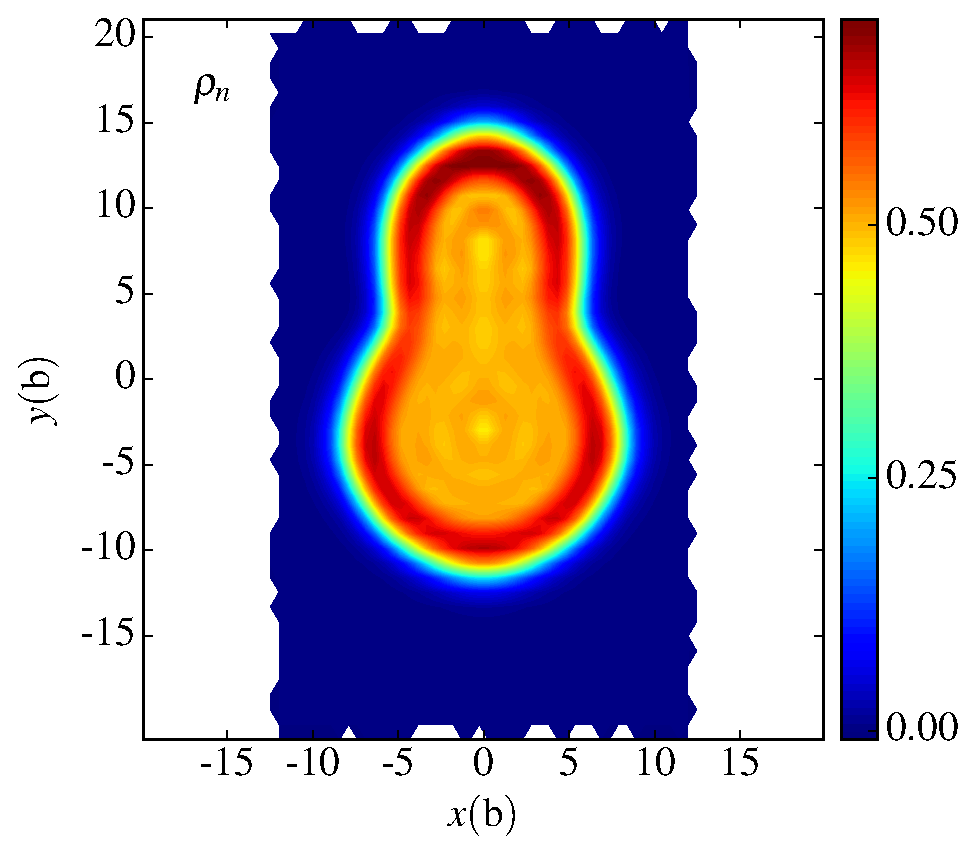
\includegraphics[width=0.3\linewidth]{294Og-140024n-locali.eps}}\label{fig:294Og-140024n-locali}
    \subfigure[$Q_{20}=200 b, Q_{30}=44 b^{\frac{3}{2}}$]{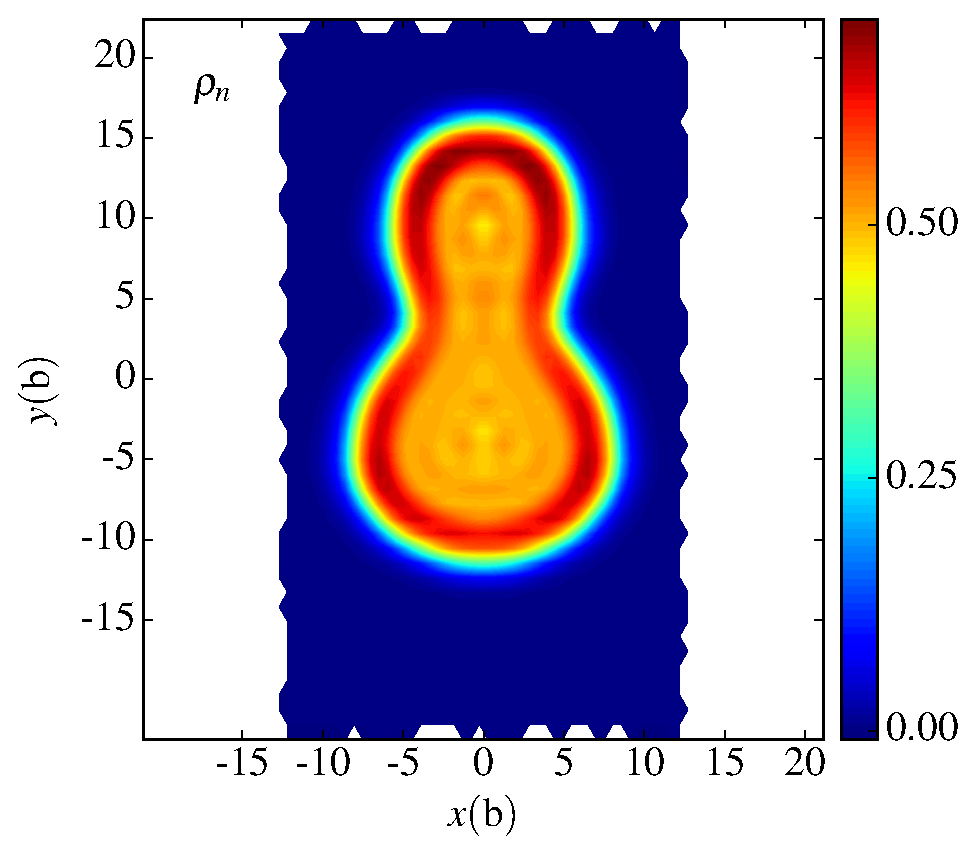
\includegraphics[width=0.3\linewidth]{294Og-200044n-locali.eps}}\label{fig:294Og-200044n-locali}
    \subfigure[$Q_{20}=264 b, Q_{30}=60 b^{\frac{3}{2}}$\newline (just before scission)]{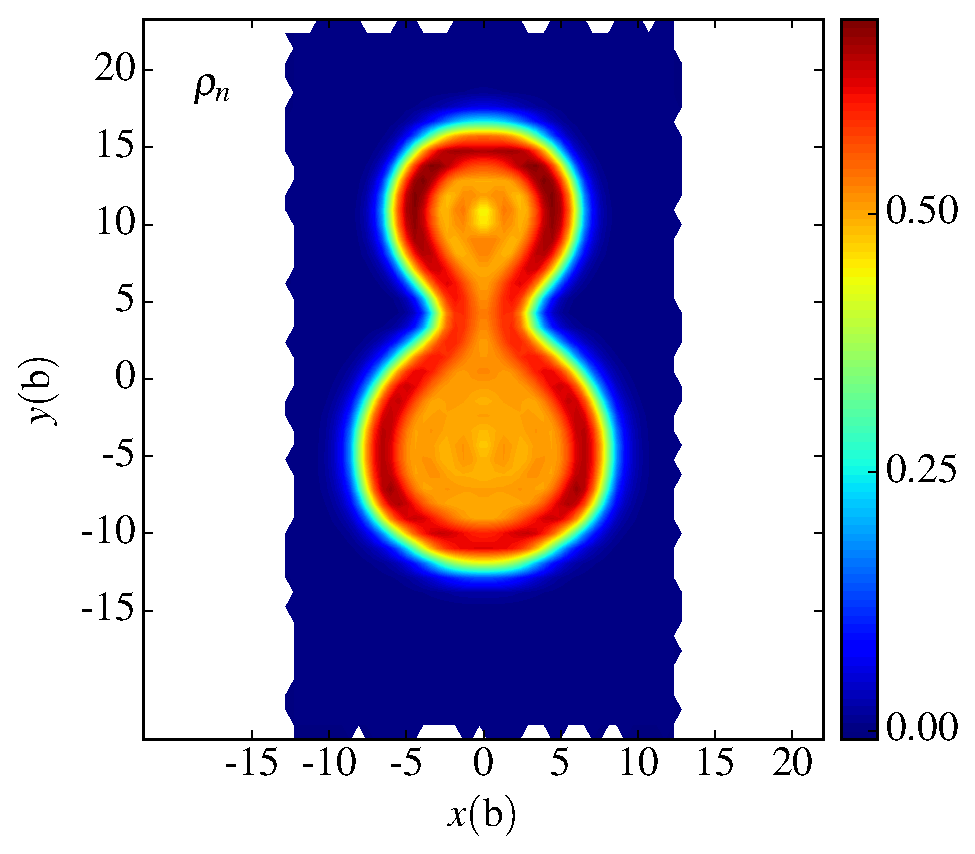
\includegraphics[width=0.3\linewidth]{294Og-264060n-locali.eps}}\label{fig:294Og-264060n-locali}  \end{center}
  \caption{Neutron spatial localization for $^{294}$Og. Shells are already starting to develop as early as just beyond the scission point}

%\end{figure}
%
%\begin{figure}[h!]
  \begin{center}
    \subfigure[$Q_{20}=140 b, Q_{30}=24 b^{\frac{3}{2}}$ (just beyond the outer turning point)]{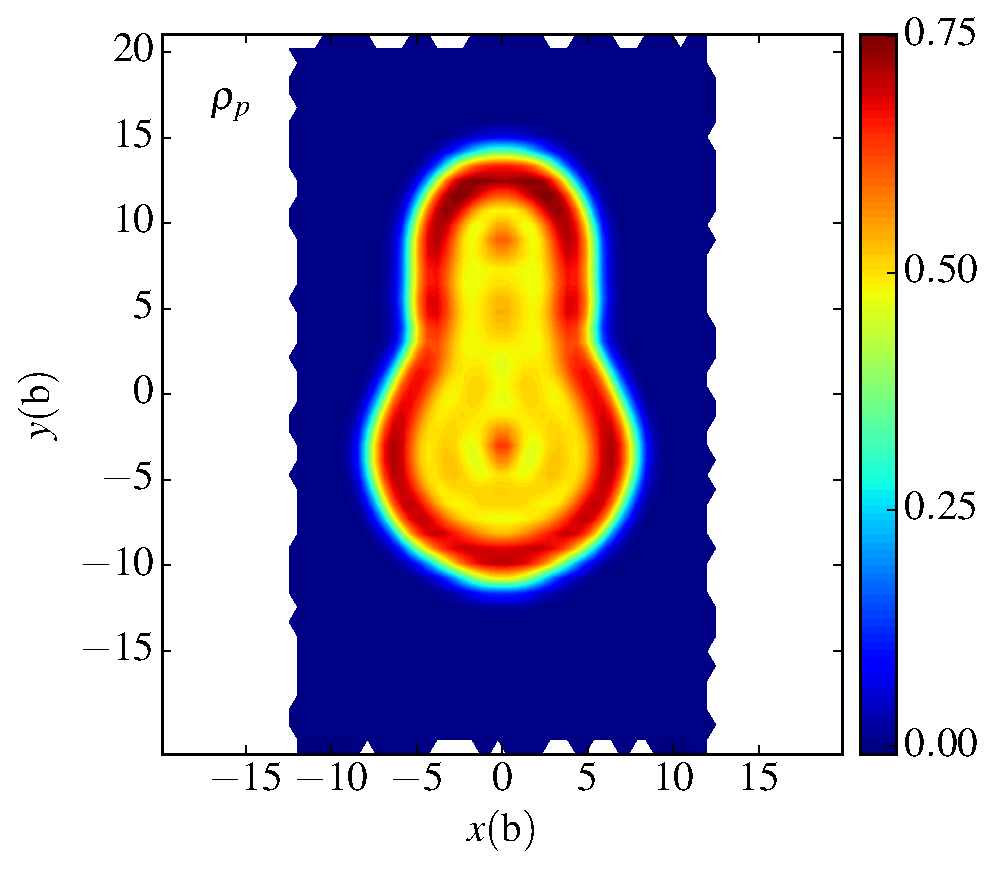
\includegraphics[width=0.3\linewidth]{294Og-140024p-locali.eps}}\label{fig:294Og-140024p-locali}
    \subfigure[$Q_{20}=200 b, Q_{30}=44 b^{\frac{3}{2}}$]{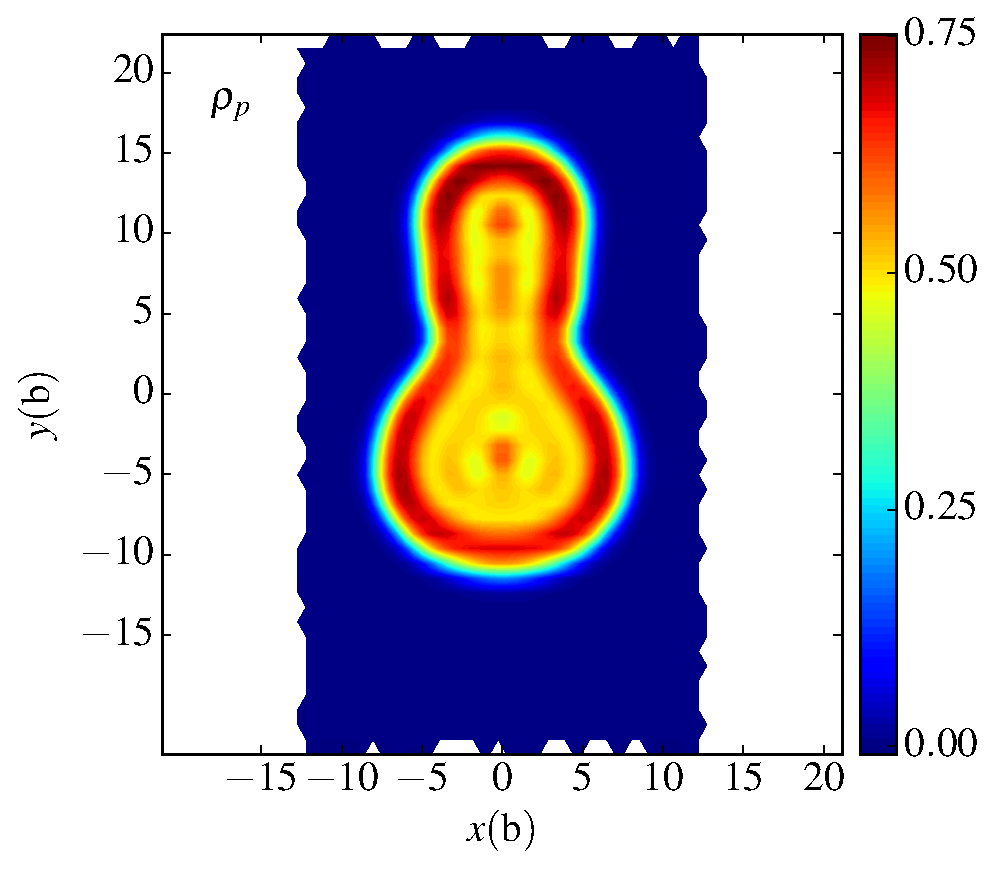
\includegraphics[width=0.3\linewidth]{294Og-200044p-locali.eps}}\label{fig:294Og-200044p-locali}
    \subfigure[$Q_{20}=264 b, Q_{30}=60 b^{\frac{3}{2}}$ (just before scission)]{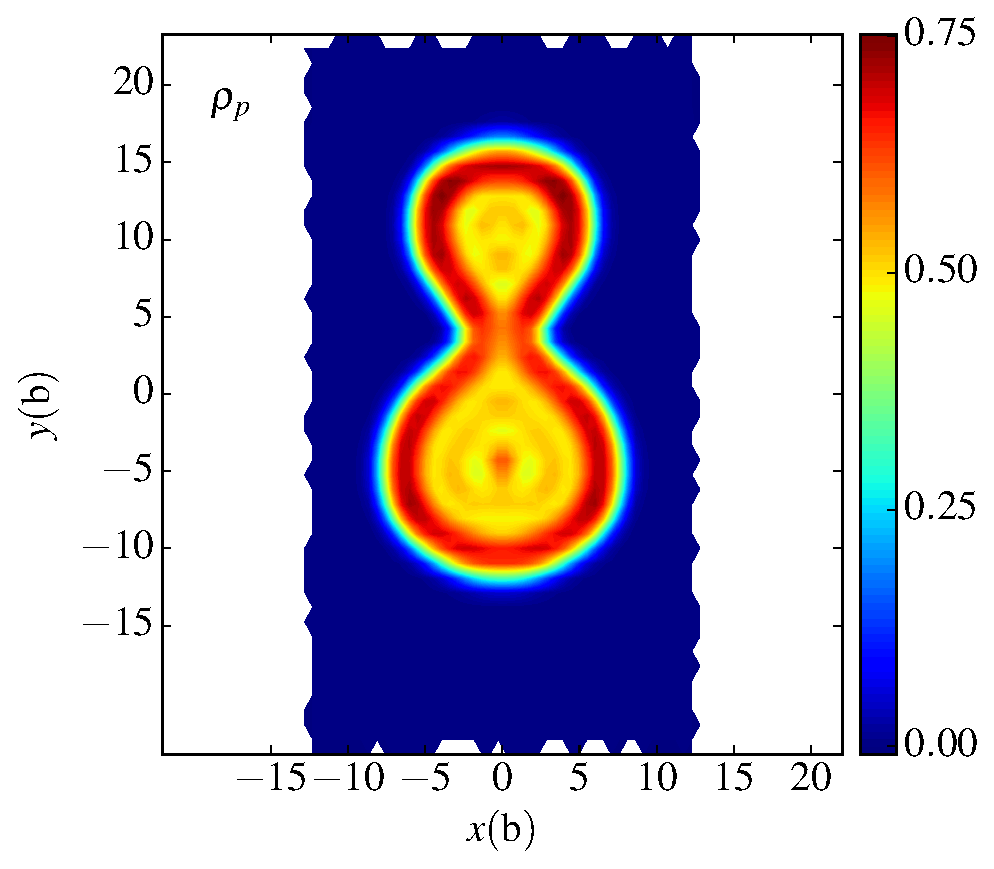
\includegraphics[width=0.3\linewidth]{294Og-264060p-locali.eps}}\label{fig:294Og-264060p-locali}  \end{center}
  \caption{Proton spatial localization for $^{294}$Og. Note that the lead proton shell starts to develop early, but the krypton proton shell doesn't develop until much later}
\end{figure}

\subsection*{2 October 2017}
One more comment I want to make clear about the plots from the previous entry: some models of cluster emission treat the system as a preformed smaller fragment trying to escape from the larger fragment. What these plots seem to show is almost the opposite, where you have a well-formed core trying to shed its excess nucleons.

\subsection*{4 October 2017}
\textbf{Re: 26 September 2017} I got back the results from giving the system a small, triaxial boost. It seems to have worked from a software perspective - they all reported back non-zero values for $Q_{22}$ - but in the end, everything still diverged. Also, it's entirely possible the boost wasn't enough - maybe there's a large triaxial barrier and $Q_{22}=3$ just wasn't enough to make it to the other side. So I guess that's the next thing I'll try. Instead of $Q_{22}=3$, I'm going to try it with $Q_{22}=30$. That might well fail, as well, just because of the jump, but it's something to try, right? And I'll do it with 10 iterations of ``pushing'' instead of 5.

\subsection*{10 October 2017}
Yeah, that large triaxial push was \textit{definitely} too much for it. Maybe if I had eased into it instead of jumping so abruptly that could have done it. But the way I did it (pushing directly from $Q_{22}=0$ to $30$) was just too much and it caused the thing to diverge after only 45 minutes (\texttt{QUABCS failed for neutrons/protons}).

\subsection*{1 December 2017}
Something that we noticed a few weeks ago was that I may have misunderstood what how $\lambda_2$ was chosen in Jhilam's \textit{Pairing-Induced Speedup} paper. I just took $\lambda_2=0$ as my baseline, but Samuel suggests that what I should have done is performed a self-consistent calculation first (with Lipkin-Nogami turned on), and then used whatever $\lambda_2$s came out of that as my baseline/zero/starting point. So now I picked a point ($Q_{20}=48, Q_{22}=15, Q_{30}=6$) and redid it with Lipkin-Nogami to use as a baseline. That converged with some values like $\lambda_{2n}=0.094, \lambda_{2p}=0.118$, which is well-within the range of $\lambda_2$-values I probed. Except that if you go to a larger value of $\lambda_2$, even as small a change as $\lambda_2=0.15$, you end up with a lower HFB energy. And worse, there seems to be a monotonic decrease at least as far as $\lambda_2=0.4$. It might start increasing again by the time I get to $\lambda=0.5$ and beyond - that's certainly what my calculation shows, but I remember being skeptical of that run for some reasons that I can't currently remember. Anyway, so I'm playing around with that, just to see if there's anything going on that we can't see somehow. So for instance, as I said I did an unconstrained calculation kickstarted with HFBTHO; now I'm using that record file to start a run using  $\lambda_2=0.15$ and another with $\lambda_2=0.4$. Hopefully, if the problem relates to the initial conditions (where in the variational space you are looking), that should show us.

UPDATE: I didn't let the two run to complete convergence, because I didn't want to waste resources, but the overall HFB energy for each constrained run at each iteration was significantly lower than the ``self-consistent'' solution, to at least 2 decimal points of precision.

UPDATE 2: Nope, wait, I was being dumb. You maybe weren't totally wrong, per se, but a better idea would be to use a constrained calculation to force yourself into a certain region, and then release the constraint from there. That's what you tried to do in the first place. Here you're just being perhaps a bit more careful about it, hopefully.

\subsection*{5 December 2017}
Okay, I think I did it better this time. I took several points, each with the same multipole constraints ($Q_{20}=45, Q_{30}=12, Q_{22}=0$), and gave them each a $\lambda_2$ in the range $[0.0, 0.9]$ in steps of $0.1$ (and a few in the middle in steps of $0.05$). I ran those and about a quarter of them converged (the other $\frac{3}{4}$ seem mostly to have diverged chaotically). Within that group, the final total energy seems to have decreased monotonically (and it's not clearly from one specific contribution, like for example the Lipkin energy). Granted, the three that converged were the three with both the smallest value of $\lambda_2$ and the ones closest to the self-consistent solution's preferred value of $\lambda_2$; perhaps if the others had managed to converge we would have seen a minimum in the final energy, followed by an increase somewhere. But given the results I have, and the range I have, there is only a decrease in the total energy, not a minimum.

Interestingly, even though some of those points converged, I was able to take their unconverged record files and run them alongside the converged record files to let the system run to its true self-consistent solution. Almost everything converged; the few that didn't seem to have gotten stuck in a nearby false minimum. But as there doesn't appear to be a particular pattern dictating which got stuck and which ones didn't, I'm content claiming that the solution from those which converged is a ``global'' minimum.

However, if you subtract off the Lipkin energy from the total energy (see eqn 6.1 in my notes, or roughly I-9, VI-96 in the original HFODD papers), you see that the total energy \textit{before} the Lipkin-Nogami correction bottoms out around the self-consistent minimum value of $\lambda_2$ (of course, there will also be a slightly different self-consistent minimum if you run the code without Lipkin-Nogami or dynamical pairing [$\lambda_2=0$]).

\subsection*{5 February 2018}
It's been a while since I wrote, but I've got some things worth recording.

As far as I can tell, I have a minimum-action pathway/half-life code that seems to do a reasonably-good job finding minimum action pathways, but a less good job finding half-lives. It still isn't a totally-settled deal - one thing we can adjust is the zero-point energy or the energy of the ground state. Changing the $E_0$ which appears in the action integral by something like 0.1 MeV can alter the half-life by a factor of like 2 or 4 (depending which way you go). Not enough to account for my results, unfortunately, but something (and actually, in the case of oganesson, it might change my results in the opposite direction to what I need).

One problem we encountered was that we were getting $M_{eff}<0$ at some points, which is of course ridiculous! Presumably these points correspond to some kind of level crossing between points on the potential energy surface (recall that components of the inertia tensor were computed using finite differences). There are probably a number of ways I could have resolved the issue (apparently Jhilam just replaced the negative values with zeros, which makes me just a little uncomfortable), but I settled on writing a Python script that checked the value of $M_{eff}$ along each possible direction (as determined by the action minimization code using chiefly the parameters \texttt{b\_span} and so on). If a point has $M_eff\geq0$ along every possible trajectory, it is rewritten into a new, filtered input file; otherwise it is discarded. This unfortunately eliminates roughly $\frac{3}{4}$ of the data I collected. I can still use my full interpolated PES by running the code first using the unfiltered input file, saving \texttt{EHFB\_int.out}, and using it to jumpstart the next run, but unfortunately a lot of that inertia data is simply lost to time. It might be worth seeing which points I do manage to keep, in order to know if my subsequent inertia is reasonable or not. That would be a good thing to check.

In any case, using the inputs as presently constituted, I computed the half-life (and the pathways) in 2-, 3-, and 4-D space using the collective coordinates $(((q_{20},q{30}),q_{22})\lambda_2)$. The results I get currently are:

\begin{list}{}{Half-lives in 2, 3, and 4 dimensions:}
\item 2D $(q_{20},q_{30}); q_{22}=3, \lambda_2=0$:    1305504.9263348267     
\item 3D $(q_{20},q_{30},q_{22}); \lambda_2=0$:    3.8268163795048664E+022
\item 3D $(q_{20},q_{30},\lambda_2); q_{22}=3$:    9.4084322399806967E-012
\item 3D $(q_{20},q_{22},\lambda_2); q_{30}=0$:    4.9637739301242774E-011
\item 4D $(q_{20},q_{30},q_{22},\lambda_2)$:       3.8820411419017089E-012
\end{list}

\subsection*{6 February 2018}
I plotted the inertias that made it through the filter (in particular, in the 3D case). There's enough to capture sort of the bulk properties of the PES, but it depends on which layer (which value of $q_{22}$) you're looking at. The parts that I'm most worried about are probably the barrier(s), and you can kind of see them but not in any clear detail. Is that enough? I dunno. I don't even know what that means...
\begin{figure}
\centering
\includegraphics[width=0.9\linewidth]{post_filtering_nans}
\caption[Points with $M_{eff}>0$]{Points with $M_{eff}>0$ (and all NaNs filtered out) shown for several values of $q_{22} (q_{22}=3,24,36,45)$}
\label{fig:post_filtering_nans}
\end{figure}

\subsection*{7 February 2018}
My abs are so sore! But that's not relevant...

I did the 4D path calculation again, but this time I added/subtracted 100 keV to the ground state energy in the action integral to see the effect on the half-life. Pretty much as expected, but now I know. The problem, though, (and as I may have said before) is that my half-life is already too small. Increasing $E_0$ (which is what Witek suggested doing) just makes it smaller.

Just out of curiosity, I also decided to try out my alternative way of computing the tunneling probabilty. That, too, is shown below.

\begin{list}{}{Half-lives with different ground state energies:}
\item $\sqrt{V-E_0-0.1}$:    4.5456834751698960E-013
\item $\sqrt{V-E_0}$:    3.8820411419017089E-012
\item $\sqrt{V-E_0+0.1}$:    1.9654750844481639E-010
\item $\sqrt{V-E_0+0.5}$:    4.8651043198529695E-007
\item Alternative tunneling prob.: Nonsense. It really depends a lot on your choice of $E_{ZPE}$
\end{list}

Also perhaps worth noting is the fact that the minimum action trajectory sometimes changes depending on your ground state energy offset. Most of them claim to stay fairly mass-symmetric and very triaxial (Really? Huh. That's interesting), but there are exceptions.

\subsection*{5 April 2018}
Samuel generated a 2D PES for $^{294}$Og using the Gogny D1M force using a perturbative recipe for the inertia. Using the values he gave me I computed a value for the half-life of Oganesson:

\begin{list}{}{Half-life in 2 dimensions from Gogny:}
\item 2D (no ZPE) $(q_{20},q_{30})$:        30786236776.996628 (3.1x10^10)
\end{list}

I'm running into some kind of problem when I try to add in the ZPE, which may owe to the fact that apparently I don't know what the ZPE is after all. Also, when I compared Samuel's input data to my own, I noticed that while $M_{q2q2}$ is of approximately the same magnitude in both cases, the other two components are roughly an order-of-magnitude larger in my file than in his. What's up with that? Did I convert from Fermis to barns wrong with Samuel's data? Or did I do something dumb with my data? Or are the data really just that different?

\subsection*{11 April 2018}
I added a little workaround in order to use ZPE corrections to the ground state (the real fix is going to take a little bit of work, though nothing too terrible). With a ZPE correction of 0.5, I now get:

\begin{list}{}{Half-life in 2 dimensions from Gogny, take 2:}
\item 2D (ZPE=0.5) $(q_{20},q_{30})$:        9837943407.0663910 (9.8x10^9)
\end{list}

Sooo... Slightly-better...

Importantly, though, the exit point changes significantly with that correction, though. Before, it was exiting along the symmetric path. But with the added 0.5 MeV correction, it now exits along the cluster path. Interesting...

\section*{How to compute half-lives}
\subsection*{20 June 2017}
I'm trying to think about things to do to improve the half-life calculation. I talked a bit before (I think) about how small changes in the factor $\delta q$ used for the finite-difference approximation of the derivatives we need to compute the inertia can eventually lead to errors as great as two orders of magnitude in the half-life. And just in general, half-life calculations are not notoriously great. So what can we do to nail down some better certainties there? Well, hammering down on the precision of those derivatives is a good start (and it seems like it might provide a way to estimate uncertainties).

Another possible fix might be to adjust that factor $n=10^{20.38} s^{-1}$ that just gets taken for granted. It could be that it's a good estimate, but that's something I'd like to decide for myself. I bet we could come up with a better estimate that is elongation-dependent (or perhaps even more complicated, but that seems like the best next-to-leading-order approximation).

A third possible space for improvement is with the WKB approximation. The WKB approximation breaks down near the turning points. There are people on the internet who have devised workarounds:

\begin{enumerate}
\item \href{http://www.physicspages.com/2014/07/03/wkb-approximation-tunneling/}{Derivation of WKB approximation}
\item \href{http://www.physicspages.com/2014/06/30/wkb-approximation-alternative-derivation/}{Alternative derivation of WKB approximation}
\item \href{http://www.physicspages.com/2014/07/09/wkb-approximation-turning-points/}{WKB at turning points}
\item \href{http://www.physicspages.com/2014/07/14/wkb-approximation-at-a-turning-point-with-decreasing-potential/}{WKB at a turning point with decreasing potential}
\end{enumerate}

\noindent One nice thing about the WKB approximation is that since it is based on a series expansion, you can estimate errors: \href{https://en.wikipedia.org/wiki/WKB_approximation#Precision_of_the_asymptotic_series}{WKB on Wikipedia}

Yet another idea is to avoid the WKB approximation altogether. You could model the barrier as a series of rectangular barriers, for which you know the exact transmission probability. The total transmission probability through the whole barrier is then the product of all the individual, infinitesimal rectangular barriers. You'd need to use a ``product integral'' instead of the usual summation integral, and even then I'm not sure you could generate an analytic expression without knowing the analytic form of the potential. But numerically, I think you'd actually be fine, come to think of it. You could basically just change or add a couple of extra terms to your path program and I think it would work just fine. In fact, once I get the path program working, I think I'll do just that!

\subsection*{29 June 2017}
Just to make sure I have it somewhere, the formula for computing the tunneling probability through a rectangular barrier of width $a$ is

\begin{equation}
T = \frac{1}{1+\frac{V_0^2\sinh^2(k_1a)}{4E(V_0-E)}}, \qquad k_1 = \sqrt{\frac{2m(V_0-E)}{\hbar^2}}
\end{equation}

I'm not sure whether this only works for the case $E>0$. It'd be nice, on the one hand, to rescale everything to some zero-point energy defining your ground state. But then your particle has zero energy, which removes all the interestingness of the expression.

\section*{Minimum Action Path}
\subsection*{4 December 2017}
I'm noticing now just how long it's going to take to compute a minimum action pathway in 4 dimensions inside the $^{294}Og$ barrier. I've left the thing running for at least 80 hours on 14 cores on iCER and it's only up to about $Q_{20}=25$ (it traverses the path in steps along $Q_{20}$). First of all, it actually takes a fair bit of time to even continue where it left off - far more than I feel like it should, like it took over an hour for the dataset that I had, when I feel like something like that shouldn't take more than a couple of minutes. But even after that, it still takes a long time. And I did some back-of-the-envelope math, and it makes sense: the surface I have spans $Q_{20}\in[-20,162], \lambda_2\in[40,0], Q_{22}\in[3,45], Q_{30}\in[0,45]$ - that's 14840934 points! Of course, we don't use quite all of those, since the algorithm is at least somewhat intelligent. But even still, it is possible to have a ``layer'' of $\sim40^3=64000$ points to check for a single value of $Q_{20}$ (for the method we use to find the path, I believe that is the most we can break down the problem), each with $(2x_{span}+1)(2y_{span}+1)(2z_{span}+1)-1$ ``next points'' to check.

I've been using OpenMP shared-memory parallelism thus far, but that's limited to the number of cores on a node. To do this quickly, it looks like it's going to take a \textit{lot} more processors, which means distributed memory parallelism. And actually, I was thinking, this might even be a case where GPUs might be able to do the job quickly. You feed in the uninterpolated data, and then the GPUs fairly quickly should be able to interpolate the surface, and maybe even action ``steps,'' and then you can find the best path and it shouldn't be too hard by then.

\section*{Miscellaneous}
A place for all the random things you learn that you don't necessarily have a place for elsewhere in the notes, but you want to put them somewhere. Like the days when you read a lot of papers and you don't want to forget what you've learned.

\subsection*{3 October 2017}
One paper I read today was about using some flow equation to derive a new nuclear energy density functional (not - so far as I can tell - based on Skyrme or Gogny [at least not yet]). The nice thing about this scheme is that it has a built in truncation scheme, which is great for uncertainty quantification and error analysis and whatnot. I don't really understand what they did but it'll be interesting to see if it leads to anything better (although looking back on it, I don't see that they've specified a potential, so perhaps we'll be stuck with Skyrme or Gogny on some level after all...) See https://arxiv.org/pdf/1709.09143.pdf

I also spent a fair bit of time reading through a paper about correlated prompt fission data in transport simulations. What these codes try to do is predict the number, energy distribution, and maybe spin/angular momentum/directional/etc. properties of prompt neutrons, gamma rays, emitted in fission, given a fragment yield and a total kinetic energy as an input (basically). The mechanism on which these codes are based is Hauser-Feshbach, which is a reactions formalism that handles compound nuclei: given some total cross section, try to reconstruct the possible input channels and their weights (or something like that). There's a lot of stuff I don't understand about it, but at least it gives me something I can refer to when people ask me questions about scission neutrons and fragment angular distributions and whatnot. See https://arxiv.org/pdf/1710.00107.pdf

I showed Witek my cluster plots for 294Og and he wasn't at all surprised that the krypton protons took forever to coalesce into their shell configuration, but he did point out what I'd already basically noticed: that it's apparently easier for heavier nuclei to emit clusters.

\end{document}          
